\documentclass[12pt, titlepage]{article}

\usepackage{fullpage} %full page typesetting
\usepackage{setspace} %allows for non-singlespacing
\usepackage{graphicx} %graphics capabilities
\usepackage{latexsym} %extra symbols
\usepackage{rotating} %rotation for figures
\usepackage{longtable} %tables that fill more than a single page
%\usepackage{hyperref} %hypertext links in the document
\usepackage{natbib} %better bibliographies
\usepackage{authblk} %author and affiliation in opening
\usepackage{mathpazo} %use palatino font, rather than times
\usepackage{appendix}
\usepackage{lscape}
\usepackage{tabulary}
\usepackage[nottoc]{tocbibind}
\usepackage[colorlinks=true,linkcolor=blue,citecolor=cyan,urlcolor=red]{hyperref}
\usepackage{ifthen}
\usepackage{float}
\usepackage{subcaption}
\usepackage{mwe}
\usepackage{caption}


\title{\tb{Place of Residence and Political Attitudes in Democracies Worldwide }}

\author{Jennifer Lin}
\affil{New College of Florida}

\newcommand\e{\emph}
\newcommand\tb{\textbf}
\newcommand\un{\underline}
\newcommand\txt{\texttt}

\doublespacing 

\begin{document}

\begin{singlespace}
\maketitle
\end{singlespace}

\begin{center} %center text
\section*{Abstract} %the star stops this section from appearing in the ToC
	
\begin{quote}
After the 2016 election, many major new pundits pointed at Rural America as the major source of Donald Trump’s victory for the presidency. This is because, as prior research by \cite{walsh_putting_2012} for the United States and \cite{walks_city-suburban_2005} for Canada suggests, residents in rural parts of democratic countries tend to be more religious and less exposed to diversity as their urban counterparts. As a result, they are more conservative in their social views even if they may be more liberal on their fiscal ones. President Trump took advantage of this and won the hearts and minds of many voters in the Midwest and Rural South, which allowed him to secure an electoral college victory despite falling short on the popular vote. For this research project, I was interested to see if this trend extends to other developing and consolidated democracies in the world. Using the CSES Module IV data (2011-2016), I conducted regressions to test place of residence on a self-defined ideological scale and an objective ideology scale constructed using respondent opinions on various issues. By controlling for regime factors such as age and level of democracy, I find statistical significance to suggest that place matters in influencing political attitudes based on the context of the country. Directions for future research in this area are fruitful as more work needs to be done to understand how the contextual forces of each polity emphasize the differences between the people's place of residence and their political attitudes.

\end{quote}
\end{center}

\clearpage

\tableofcontents
%\addcontentsline{toc}{section}{\listfigurename}
%\addcontentsline{toc}{section}{\listtablename}
\clearpage

\listoftables
\clearpage

\listoffigures
\clearpage

%\section{Introduction}

After the election of Donald Trump as the 45th President of the United States, news pundits speculate that the reason for his election was through the support that he won from rural voters in the South and Midwest. These Republican strongholds located in the rural and suburban parts of the country have been researched by political scientists \citep{walsh_putting_2012} and the results suggest that there is an urban-rural divide that is growing in the United States. Additionally, it is noticeable that the mindset of individuals who live in different parts of the country do not conceptualize politics in a similar fashion \citep{holloway_burning_2007}. These differences in interests leads to differences in ideologies and attitudes, as seen in the United States back in 2016.

However, the United States does not operate in isolation and the people are not necessarily idiosyncratic compared to others around the world. Therefore, in this paper, I am interested in understanding if the urban-rural divide that is present in the US is also present and noticeable in other places around the globe. Additionally, I  will discuss how living in a different environment leads people to favor different interests and hold distinct political beliefs in the context of key regime factors such as the level of democracy, age of regime and the type of electoral formula that a regime employs in their system of government.

Through the analysis of the Comparative Study of Electoral Systems (CSES) Module IV data, I find that place of residence does matter in influencing one's political beliefs and ideologies. More specifically, the results will allow us to draw a key conclusion: The place of residence matters in influencing political attitudes, but this is heavily influenced by regime factors such as level of democracy, regime age electoral formula, Freedom House Rating and corruption.

\section{Analysis of Previous Research}

Past research in this topical area considered the influence of place in specific case studies. These results will be analyzed in this section of the paper, followed by an analysis of general conclusions that these cases suggest. I will also briefly introduce the countries that are being included in this paper and conclude the section with a word of caution before moving to the data analysis. 

\subsection{Trends of Urban-Rural Divide in Seen in Previous Case Studies}

The most popular places where literature exists for understanding the urban-rural divide in political attitudes lies mostly in the developed world. Namely, the United States, and Canada are the top countries where this trend has been analyzed most frequently. As we will see later, these are also the two countries that do not have the full supply of data in the Comparative Study of Electoral Systems data to be included in this paper. Therefore, I will consider the lessons learned from these two places, along with some others, as a way to gain some insight on the extent of rural-urban influence on political attitude development in a developed democracy in hopes of understanding how other polities differ in their own unique ways to the conditions of the polity.

\subsubsection{The United States}

One of the earliest works in studying the influence of place on public opinion comes from \cite{glenn_rural-urban_1967}. In this study, the authors explored the extent of rural and urban differences on people's attitudes towards certain policy issues. Their findings suggest that such a difference exist such that rural residents tend to be more conservative on economic issues and more fundamentalist when it comes to religion.

In a more recent study, \cite{gimpel_rural_2006} examines the divide of American citizens in previous US elections and found that rural and urban residents differ significantly in their social and economic views on the issues. Rural residents tend to have a stronger sense of self reliance and tend to think that others ought to do the same \citep{walsh_putting_2012}. As such, voters in rural America are motivated to vote for the Republican party. Figure \ref{figure3} in Appendix \ref{AppendixE} shows the \cite{NYT-trump} reporting of the 2016 results by county. This graphic reflects the prevalence of voters in the rural parts of the United States helping Trump carry his electoral victory. As a result, we see that there is a divide between place of residence and political views in the United States.

\subsubsection{Canada}

Elections in Canada follow a similar pattern to the trends noted in the United States. While it is a younger democratic regime in comparison and has representative that are elected via a proportional representation system, research in Canadian elections starting in 2003 suggest that the divide between place of residence is present and exacerbated by party polarization in the political system \citep{walks_place_2004}. Canada's New Democratic Party selects candidates that prioritize the needs of cities, pushing voters in the suburbs and rural areas to support a more conservative, right-wing option. A time series of Canadian elections from 1945 to present also confirms this drift and divide between voters based on their place of residence \citep{walks_city-suburban_2005}.

\subsubsection{Other Countries}

In the general light, residents in one area often view a neighboring, unfamiliar region by the stereotypes that define it. In France, this is quite the case \citep{clout_new_2003}. Urban residents see the rural plains as undeveloped lands that are waiting for their entrepreneurial talents. Yet, rural interests often go unnoticed unless a party that would speak for them is in power. Yet, the people of France, on all sides of the picture, are not alone. In this section, I will consider other countries where signs of an urban-rural divide is visible and emerging. This perspective can serve as an interesting starting point for the analysis to follow in this paper.

The Liberal and Labor parties of Great Britain serve different interests with the former most favored to serve the desires of farmers. The Countryside Alliance was formed in the UK in 1997 as a means for farmers to take back their status after the domination of the Labor Party in UK politics \citep{benton_ruralurban_2007}. The people of the UK are not necessarily divided by their political ideologies; rather, they are divided by interests, which leads to different party supports for urban and rural residents. As urban residents outnumber rural residents, their interests often dominate, placing Labor in power more often than what rural farmers would agree on.

A person's place of residence is the most important gateway to the possibilities of social network formation and interaction across the globe, but this is emphasized in research done in the Netherlands. As \cite{van_gent_right-wing_2014} suggests, social networks are often tied to geography such that political socialization and attitude formation is a possible outcome of differences in electoral geography. The neighborhood is fertile ground for the clustering of social classes, leading to divisions between places of residence. While there is a clear divide between urban and rural residents for their partisan support in the 2010 elections in the Netherlands, the underpinnings of this divide are interesting to consider when conceptualizing how people vote by place.

However, when it comes to developing democracies, divisions of place is another hurdle that the polity must cross in order to achieve some form of stabilization in their regime. In Lithuania \citep{jurkynas_emerging_2004}, the divide between residents is present in their support for the Peasant People's Party. Rural residents throw their support behind this party for their stance against the rise of landowners with the introduction of a market economy. However, in the context of post-communist states, research also notes that there are other hurdles that may be harder to cross than a rural-urban divide. Conflicts between ethnic groups and political actors may put more pressure on the establishment of a stable democracy. 

From this sampling of countries, the rural-urban divide does not seem to be solely a phenomena of the United States. Not only is this difference present, it also plays a role to influence individual attitudes and trust in the government \citep{ahn_political_1986}. 

\subsection{Connections between Place and Political Ideology}

Previous authors analyzed in this paper have considered the presence of underlying factors that influence the apparent urban-rural divide in electoral behavior. However, what are these possible connections and how do they matter? 

To begin, the link between place and political ideology varies with the qualities of the individual \citep{orbell_impact_1970}. Education, income and previous places of residence, among others, shape the individual's course of live and exposure to information and additional political ideologies and attitudes. This is seen in a case study of the people of Zimbabwe's Eastern Highlands \citep{moore_subaltern_1998}. Here, people developed attitudes towards their country and government based on the ways that they were raised and the varieties of environments that they had been exposed to as they grew up. Familial socioeconomic factors would proceed to influence the ways that these lessons and views would be passed down to their children, and shared with the village. 

While personal factors matter to determine the development of one's morals and perceptions of political efficacy, comparative case studies on six European countries suggest that trends of globalization, along with its components of economic and social competition, can influence not only the development of a party system in a country, but also shape the viewpoints of the people in it \citep{kriesi_globalization_2006}. When party systems developed during European countries' transition to democracy, the people were lined on interests based on their stance on economic and social issues. As \cite{walsh_putting_2012} implies, place influences one's development of their stances on these issues, thereby leading place of residence to have the potential of influencing the survival of political parties.

In general, the possibilities of social interactions between people in a specific vicinity matters in how they will form their political attitudes. Early research in this field \citep{glenn_rural-urban_1967} shows that rural residents are less trusting of their neighbors than their urban counterparts.  In a more recent study using 2000 Census data in the United States, the research suggests that diversity is a great factor influencing liberal views, or lack thereof \citep{williamson_sprawl_2008}. When people are in places where diversity is vibrant, they are more likely to be open to newer experiences. Yet, this is most likely, in modern times, an occurrence of the urban centers and less so once one moves to the margins of geographic space in society. Therefore, space matters in the opportunities for attitude development because it facilitates one's exposure to diversity and opens the door to possibilities. Yet, at the same time, the state of development of the country on it's path to democracy, along with the political participation of the individual residents, also contribute to the connections between place of residence and political ideology. Therefore, the connection between place and political attitudes rests both in the upbringing of the individual, their opportunities, and the development factors that surround the country that they live in.

%%%TEASE out this section a bit more to add the explaination for why diversity in urban centers would make it more likely for them to be more liberal.

%\subsubsection{A Note on Psychological Place-Based Attachments}

%\subsubsection{Neighborhood Social Groups and Political Affiliations}

\subsection{Polities in this Study}

The Comparative Study of Electoral Systems (CSES) database was launched in 1996 and is a center for data collection of different polities worldwide. Thousands of respondents are interviewed per election cycle in each of the countries and their responses are aggregated to form the dataset that is used for this experiment. This section is a brief overview of the elections that are considered in the Module IV dataset.

%Table for D2031 by polity

Table \ref{table2} shows the percentage of people in each polity that lives in each of the four different places of residence. This table provides context for the specifications in each country that should be factored into account when we conduct the analyses. Based on geographic factors and economic trends, residents of some countries may find it more beneficial to flock to a certain regions of the country for personal political or economic gains. Additionally, factors relating to a country's level of development may influence the distribution of where people live such that it plays to influence their political stance. 

\begin{table}
	\centering
	\caption{\tb{Percentage of People in Each Place of Residence by Polity}}
	\begin{tabulary}{\linewidth}{l c c c c}
		\hline
		\tb{Country}&\tb{Rural}&\tb{Small Town}&\tb{Suburban}&\tb{Urban}\\
		\hline
		Worldwide&26.98&22.95&13.37&36.70 \\
		Argentina&-&13.30&-&86.70 \\
		Australia&10.92&18.73&16.98&53.37 \\
		Austria&41.67&27.54&18.19&12.60 \\
		Bulgaria&26.33&20.82&36.14&16.72 \\
		Czech Republic&26.68&39.87&5.01&29.24 \\
		Germany&28.80&42.56&9.53&19.11 \\
		Finland&25.16&23.39&42.50&8.95 \\
		France&35.10&37.34&11.72&15.84 \\
		Great Britain&17.68&52.84&-&29.48 \\
		Greece (2012)&40.77&10.62&11.51&31.10 \\
		Greece (2015)&5.86&21.48&13.99&58.68 \\
		Iceland&9.06&28.87&26.17&35.90 \\
		Ireland&-&40.91&-&59.09 \\
		Israel&20.50&54.40&25.10&- \\
		Japan&12.80&25.86&17.86&43.47 \\
		Kenya&66.67&-&-&33.33 \\
		Latvia (2011)&36.75&18.13&-&45.12 \\
		Latvia (2014)&34.46&25.29&10.42&29.83 \\
		Mexico (2012)&18.33&11.67&-&70.00 \\
		Mexico (2015)&18.38&11.28&-&70.34 \\
		Montenegro&37.47&36.72&12.85&12.96 \\
		Norway&26.43&25.54&13.69&34.35 \\
		New Zealand (2011)&16.32&38.12&-&45.56 \\
		New Zealand (2014)&13.36&21.04&-&65.61 \\
		Peru&20.99&-&-&79.01 \\
		Philippines&45.00&14.58&3.33&37.88 \\
		Poland&35.85&42.57&9.64&11.93 \\
		Portugal&28.75&25.48&16.81&28.95 \\
		Romania (2012)&44.63&22.83&2.37&30.97 \\
		Romania (2015)&41.82&29.95&11.78&16.46 \\
		Serbia&49.62&24.04&9.44&16.90 \\
		Slovakia&42.38&39.16&1.48&16.97 \\
		Slovenia&22.88&12.65&49.66&14.61 \\
		South Africa&30.77&-&-&69.23 \\
		South Korea&17.00&28.40&6.00&48.60 \\
		Sweden&17.55&22.12&21.15&39.18 \\
		Switzerland&26.67&0.66&47.30&25.37 \\
		Turkey&19.06&21.64&17.96&41.34 \\
		\hline
	\end{tabulary} \\
\e{Source:} Comparative Study of Electoral Systems Module IV 
\label{table2}
\end{table}

%Thailand&76.24&3.61&4.08&16.07 \\
% Figure \ref{figure1} provides a general overview of the place of residence of the respondents for the data used in this study. At an instant glance, it may appear that the urban residents are oversampled, but considering that, as Table \ref{table2} suggests, more people live in urban centers than suburban areas, it balances out to represent the world's populations on a general trend.

%\begin{figure}[ht!]    \centering
%	{	 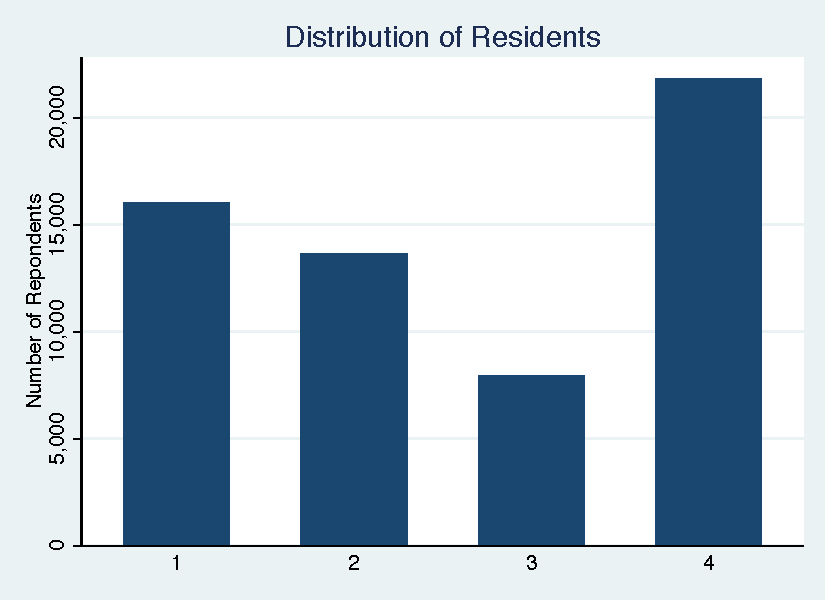
\includegraphics[width=\textwidth]{Residents}}
%	\caption{\tb{Distribution of Responses By Place of Residence}}\label{figure1}
%\end{figure}

In addition to the distribution of residents, it is also beneficial to note some of the macro trends that are present which can help categorize the countries and take their variations into account in the analysis. As we will see later, I use the CSES variable for democracy but also include several other factors to check the definition of democracy to be as close to how \cite{diamond2004overview} categorizes its key characteristics -- regimes that grant citizens individual freedoms, equality before the law and feature government responsiveness.

\begin{figure}[ht!]    \centering
	{	 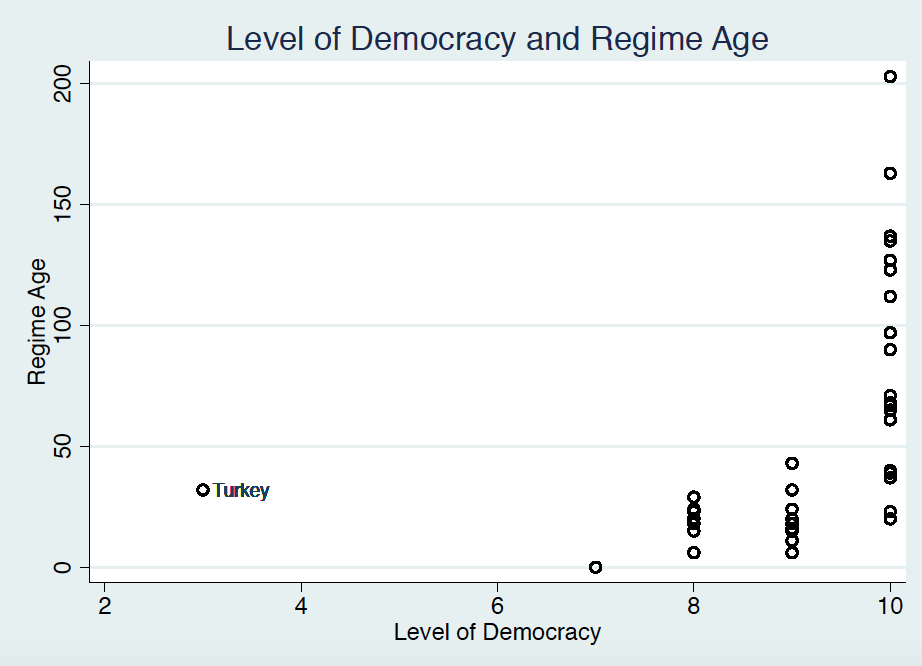
\includegraphics[width=\textwidth]{AgeDemPF}}
	\caption{\tb{Level of Democracy and Regime Age}}\label{figure2}
\end{figure}

Figure \ref{figure2} shows a graphical display of the countries represented in Module IV of the CSES sorted by their level of democracy and regime age. As the graph suggests, most of the countries represented in this study are very free. Yet, when it comes to the time that the electoral democracy has been around, most reside under the 50 year mark but it largely centers around and below 25 years. Table \ref{table101} in Appendix \ref{AppendixC} shows this data broken down more specifically, adding the consideration of the regime's electoral formula. 

From what this figure can show us, it is important to note some extreme values on both variables. Turkey's 2015 election stands out on Figure \ref{figure2} because it is the least democratic of the group. Additionally, it is also interesting to note the longest standing democracies such as the United States, Switzerland, Australia, Canada and New Zealand. These countries are those where there are most prior research given the country's openness to gathering of data from its citizens and the people's abilities to express their desires freely. The countries that center around eight and nine on the democracy scale that have democracies that are younger than 50 years will be the most interesting to consider given limitations in the existing literature that is available for these places.

\subsection{Proceeding with Caution}

As seen in previous works in American and Canadian politics, political parties are useful tools to predict votes since they are relatively useful heuristics that can assist in the formation of voting blocs. However, as \cite{holloway_burning_2007} notes, place of residence is not uniform throughout the world and it's people should not be treated as such. Rural voters are not voting blocs even if they can be seen to have similar voting patterns that span across a period of time. Yet, while some conceptualize a group under one light, it is not entirely the most accurate description of the way this group operates. Therefore, in answering the question of how place of residence influences political attitude formation, I aim to understand the general trends that happen in the world as a whole, but also within the boundaries of each country. I wish to tap into underlying mechanisms that can provide insight to why these trends exist and its repercussions in the hearts and minds of fellow citizens. I do not aim to make voting predictions about a country's next election; rather, I seek to understand if living in a place, on average, influences vote choice based on availability of social resources and activation of personal interests. With each of the conclusions I draw, the literature suggests that there are variations and other noise factors that should be considered before seeking to make generalizations about the rural or urban place of residence as a whole.

\section{Hypotheses}

From the review of literature, we see that there seems to be an ideological divide between people living in rural and urban areas of their respective countries. From case studies, most notably in the United States and Canada, there is a pattern such that the individuals living in rural areas tend to err towards conservatism and residents of urban centers tend to veer towards liberalism. However, given that these are relatively established democracies, I wonder how differences in levels of democratic development, regime age and other idiosyncratic factors that shape a regime influence the divide of political ideologies between urban and rural residents. Therefore, the present research will test three hypotheses relating to the relationship between the place of residence of an individual and their political ideology. For each of the following hypotheses, I address them as they speak to the average trends but also specific trends for each country analyzed.

\begin{quote}
	\e {Hypothesis 1 -- Self-Identified Ideology:} An individual's place of residence influences their political ideology such that the more distant the characteristics of one's vicinity gets from an urban city, the more conservative one will become.
\end{quote}

The \e{Self-Identified Ideology} hypothesis suggests that there is a direct relationship between place of residence and political ideology no matter where an individual lives in this world. Therefore, this hypothesis assumes that, broadly speaking, individuals who live in a rural area will be more conservative than those who live in a small town or urban center. In this case, political ideology, as we will also see later, is operationalized by the respondent's self-placement on the ideology spectrum. Therefore, this is based on their own views on how liberal or conservative they are. While this is helpful to understand how place of residence influences political ideology, it would be even more helpful to introduce a second hypothesis that looks at objective support for policies which can show where a person lies on the political spectrum.

\begin{quote}
	\e{Hypothesis 2 -- Issue Stances:} An individual's place of residence influences the way they conceptualize pressing issues and their stances towards these issues.
\end{quote}

In the \e{Issue Stances} hypothesis, I predict that people will understand the meaning of issues differently based on where they live and hold different opinions about them as a result of their place of residence. In other words, if the \e{Self-Identified Ideology} hypothesis holds true, people who live in rural areas will see issues differently than those who live in urban areas and apply their political ideologies when deciding on the issues. 

Both the \e{Self-Identified Ideology} and \e{Issue Stances} hypotheses assumes that countries are the same across the board and that one's conceptualization of place of residence is uniform. Therefore, in the last hypothesis, I will integrate some polity defining factors into the model to understand how certain aspects of each regime such as their level of democracy, regime age and electoral formula influence the relationships that are observed in the preceding hypotheses. 

\begin{quote}
	\e{Hypothesis 3A -- Level of Democracy:} A regime's level of democracy will influence the political ideologies of citizens based on their place of residence such that the influence of place on political ideology will increase as a regime becomes more democratic. 
	
	\e{Hypothesis 3B -- Regime Age:} A regime's age will influence the political ideologies of citizens based on their place of residence such that the relationship between place of residence and political ideology will be more pronounced when the regime is older
	
	\e{Hypothesis 3C -- Electoral Formula:} A regime's method of elections will influence the political ideologies of citizens based on their place of residence such that pluralistic, first past the post systems will increase the influence of place of residence on political ideologies.
	
	\e{Hypothesis 3D -- Polity Differences:} The regime's level of democracy, age and electoral formula will cooperate to determine the extent to which place of residence can influence political ideology in a given polity.
\end{quote}

Each of the components embedded in Hypothesis 3 analyzes key differences in how each polity functions and the stability of democracy such that a more stable democracy can mean more room for an individual to consider their true self-interests rather than being forced to believe something as a means of survival. In each of the sections of Hypothesis 3, we analyze how the successful consolidation of democracy, or lack thereof, influences how other social factors, such as place of residence, can influence a person's political views. I include the age of the regime to identify if a longer lasting polity can solidify the patterns of influence that place of residence has on an individual's political outlook and stance on issues. 

Finally, I include the electoral formula as a means of understanding how the system of representation influences the relationship between the core variables used in this paper. A regime's electoral formula is the way in which citizens select their representatives and the mechanisms in which votes are tallied. It is unclear whether the electoral formula influences political discourse and attitude formation. however, past research suggests that this factor does not matter in the ways that place of residence will influence a person's political preference \citep{barkan_space_2006}. For the \e{Electoral Formula} hypothesis, I hypothesize that if individuals had to fight for representation in a winner take all system, personal factors such as place of residence will be more salient than if all interests were more fairly represented in a proportional system. Each of these components are then tied together to understand how idiosyncrasies of a polity lead to the difference between place of residence and political ideology as explored in the \e{Self-Identified Ideology} and the \e{Issue Stances} hypotheses.

Through the research, we will be able to see whether there is a relationship across the globe surrounding place of residence and political ideology. In the following sections, I explain the models that will be used to understand the relationships between the variables. We will revisit the hypotheses in the discussion to see if the data supports them along with possible limitations that may be present.

\section{Research Design}

\subsection{Data}

To understand the divide between rural and urban residents in different countries of the world, I will consider cases analyzed in the Comparative Study of Electoral Systems (CSES) Module IV dataset for the analysis of these trends. In this specific module, the CSES considers elections that occurred between 2011 and 2016 in various democracies around the world. In the following sections, I will describe the variables used in this project in more detail. Each of the variable names and descriptions are also located in Appendix \ref{AppendixA}, which contains the variable code referenced in the CSES dataset.

\subsection{Key Independent Variables}

In this data analysis, the key independent variables that are considered include the respondent's country and place of residence. For this analysis, place of residence is considered to be based on the categories that are established by the survey such that individuals either live in a rural village, small town, suburbs of a large city or within the large city itself. In the regression model, this variable is characterized as a category even though there are places that may be in between two of the categories that characterize place of residence. 

The coding of a place of residence largely lies in the hearts and minds of the individual respondent. While the CSES works to define the circumstances that will differentiate one region from another in order to standardize the results, there are, nonetheless, both individual and country differences in codifying the definitions of each place. For example, the definition of urban in Japan is any place with more than 200,000 people whereas in Israel, an urban place of residence means that the respondent lives in Tel-Aviv, Jerusalem, or Haifa. Rural areas are often more uniformly defined as any place, once translated from the language of the survey, to be an area sparsely populated. 

Each individual's country of residence is also classified based on the year of the election, level of democracy during the election year,  age of the current governing regime in the country at the time of the election, and the type of electoral formula employed by the governing body to determine winners of seats in government. The level of democracy is characterized by the functions of the ability for people to govern at the time of the election. This measure was gathered from the generators of the Polity IV project and reflects democratization from a -10 to 10 scale with -10 being the most autocratic and 10 being the most democratic. The definition of democracy used in this measure largely follow the \cite{linz1996problems} conceptualization as the ability for the regime to hold free, fair, open and competitive elections to select leaders on the central government. The age of the current governing regime suggests how long the current system has been in power. The larger value suggests that the current system in government has been established for a longer period of time and is therefore more stable. Finally, the type of electoral formula describes how government official win office based on their total vote share. Contestants may win via majoritarian, proportional or mixed system. 

As a way of furthering our understanding of the way democracy is defined within the context of each country and with the model proposed by \cite{diamond2004overview}, I also include the Freedom House Rating and the aggregated level of perceived corruption within each country to understand the extent of individual political freedom, equality before the law and government responsiveness. These variables both serve as added independent variables and controls but do not have hypotheses attached to them. Their inclusion is to check the Polity IV rankings and to seek to understand the relationship between the factors relating to the state of democracy in each regime.

%Add controls for Gender (D2002) , Age (2018-D2001_Y) and Socioeconomic status (D2012)

\subsection{Key Dependent Variables and Measures}

To understand where individuals see their own political values, the dependent variable reflects their self-identified ideology, a variable coded by the CSES that ranges from 0 to 10 with 0 being the most left leaning and 10 as the most right leaning ideological stance. Since this can be rather subjective, I also created a liberalism/issue stances scale that reflects individual values on government spending with a more liberal vision being those who value spending for social benefits and a more conservative view for those who do not with for such spending or for those who wish to spend more to boost defense as a means to secure their country's identity and values. (See Appendix \ref{AppendixB} for a more detailed description of this scale creation) This 9-point scale was generated from questions relating to public expenditure used in the survey. Topics for these questions include health, education, unemployment benefits, defense, old age pensions, business and industry investments, police and law enforcement and welfare benefits. Additionally, I add a value of economic equality to the measure as a means of understanding how each person values equality as part of their ideological outlook. This scale ranges from 0 to 9, with 9 being the most conservative and 0 being the most liberal. In the broadest context, respondents who score at the extreme ends of the scale are seen to be most conservative or liberal in terms of their outlook on spending, which can speak to their views on social values given their willingness to allocate government money to these groups.

\begin{figure}[ht!]    \centering
	{	 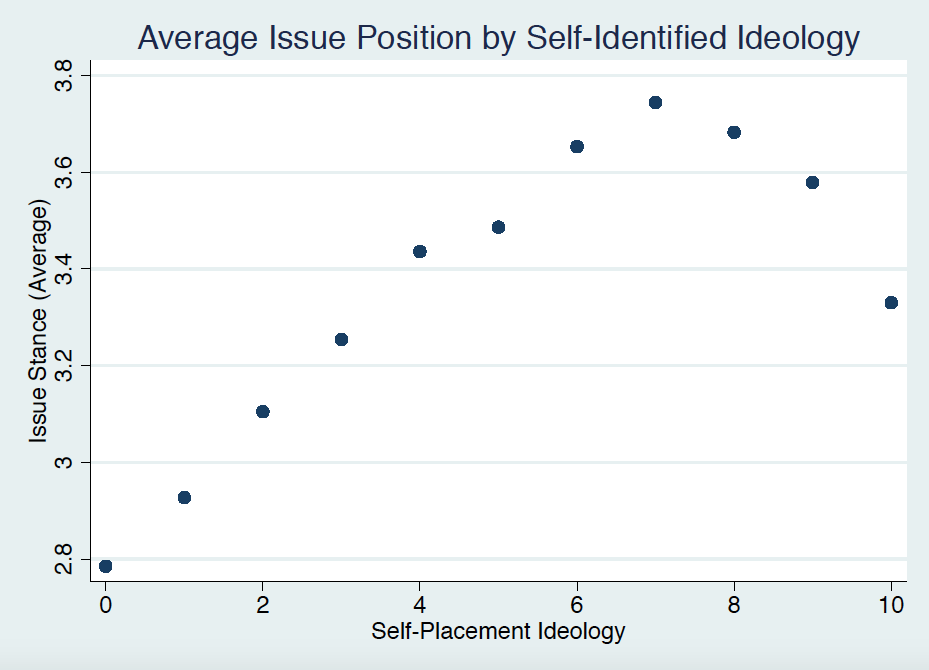
\includegraphics[width=\textwidth]{AvgLibPF}}
	\caption{\tb{Relationship between Self-Identified Ideology and Issue Stances}}\label{AvgLib}
\end{figure}

In Figure \ref{AvgLib}, the data suggests the relationship between the two variables. The graph suggests that there is a generally positive relationship between the variables and it tapers off followed by a fall at point 7 on the self-placement scale. Based on this general overview, it suggests that the people who see themselves as most right leaning are actually not as conservative on government spending as they might see themselves.

\subsection{Key Control Variables}

To ensure that we are able to compare the countries and individuals purely based on the place of residence, I employ several controls to the model. These include gender, highest level of education, socioeconomic status, age of respondent, religiosity of respondent, party identification and closeness to a party. 

The gender of the respondent is a dichotomous scale of male versus female. Subjects have the opportunity to decline to respond, as they do in all other variables. Education measures the highest level of education attained by the respondent. The socioeconomic status (SES) measures where the respondent stands on the income ladder. A respondent's age is coded based on the year this analysis is conducted (2018) subtracted from their birth year. 

Religiosity is included as a control because it is often the case that more religious individuals tend to be more conservative. Therefore, this variable measures the extent to which the respondent would agree that they are religious, not necessarily which denomination they identify with. 

Party identification varies widely by country, especially based on the way it is coded in the CSES. Therefore, party ID is treated as a control in the general analysis, along with an individual's feelings of closeness to the party. 

As a result of employing these controls, the number of respondents that we can study drastically decreases from the number of available samples in the original dataset. This is because, as mentioned earlier, any respondent who refuses or does not know the answer is marked as missing data. While this method allows us to get a better picture of the relationship between place and political ideology, it systematically rules out certain countries from the picture because of non-response or lack of inclusion of a particular item in the country's version of the questionnaire 

\subsection{Models for Analysis}

In this study, I will utilize five different regression analyses for self-placement on the ideological spectrum as a dependent measure to uncover patterns in the data and help answer the guiding questions posed in the introduction. I will also use a regression to uncover the influence of each of the macro variables on the objective liberalism scale as a dependent measure. In all, I will utilize the variables discussed in the previous sections to find connections between place of residence and political ideologies.

The first regression will consider the core of the \e{Self-Identified Ideology} hypothesis. I will regress the place of residence variable on the respondent's self-placement on the political ideology scale. The second, third and fourth regressions will factor in the effects of a country's level of democracy, regime age, and electoral formula at the time of the election into the picture to observe their influences on the relationship in the \e{Self-Identified Ideology} hypothesis. A fifth regression will be employed to understand how the inclusion of all the variables influences the first hypothesis. These subsequent hypotheses are aimed at testing the components of Hypothesis 3.

Hypothesis 2, or the \e{Issue Stances} hypothesis, is constructed as an objective measure and check to the subjective ratings. The Liberalism scale will be a dependent measure on another series of regressions that mirror the first set. The major difference with this set of regressions from the preceding set is the differences in dependent measure such that the former is based on how individuals think they are placed on the political ideology spectrum based on self-judgment, the latter is the measure of ideology based on the individual's actual policy stances.

In the following section, I discuss the results for the regressions and comment on the observations that these regressions can suggest for the relationship between place of residence and political ideology across a sample of countries across the world. The discussion of countries will be broken down by general geographic region in order to understand if and how neighborhood differences influence these trends as they usually do with it comes to a country's transition to democracy \citep{brinks2006diffusion}.

\section{Results}

\subsection{Self-Placement Ideology as a Dependent Measure}

\subsubsection{\e{Self-Identified Ideology} on the Worldwide Scale}

For the first model, a regression was conducted to see if there is a general trend between place and self-placement on a 10-point ideology scale. Furthermore, the regression was conducted separately for each election that was represented in this dataset. Table \ref{table3} shows the results for this regression on the global scale. This general trend suggests that, without considerations of any polity-specific factors, there is a difference between the global rural residents, small town and suburban residents in terms of their political ideologies. The trends described in this table suggests that, on a general level, there lies a difference between where people live and their political attitudes. However, several caveats are present in this analysis. From here, we are assuming that individuals conceptualize the places of residence in a similar fashion across geographic boundaries. Additionally, this analysis does not take into account country-specific measures such as the presence of the different possibilities of residence for the people. As I noted in Table \ref{table2}, not all the countries have respondents from each place of residence as categorized in the CSES. Therefore, it would help to break down the analysis by country.

\begin{singlespace}
	\begin{table}[H]
		\centering
		%\def\arraystretch{1.5}
		\caption{\tb{Self-Placement Ideology - Worldwide}}
		\begin{tabulary}{\linewidth}{l c}
			\hline
			\tb{Place of Residence}&\tb{Worldwide} \\
			\hline
			Small Town&.1647**  \\    
			& (..0722)   \\
			Suburban & .2714***\\ 
			& (.0934) \\
			Urban   & .2679***   \\
			& (.0721)    \\
			Constant   & 5.1086***  \\
			&(.1993) \\
			N  & 10,548  \\
			$R^2$	& 0.0454 \\
			\hline                                       
		\end{tabulary}
		\\
		\e{Notes:} *p$<$.1, **p$<$.05. ***p$<$.01 \\
		\e{Reference:} A rural place of residence serves as the baseline for comparison
		\label{table3}
	\end{table}
\end{singlespace}


\begin{figure}[H]    \centering
	{	 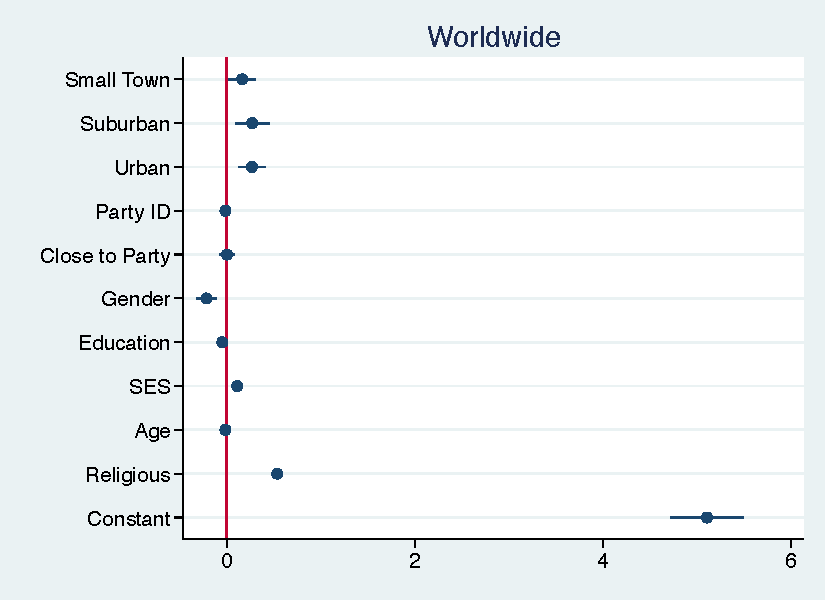
\includegraphics[width=.6\textwidth]{CoefAllIdeo}}
	\caption{\tb{Coefficient Plot for Global Ideology Trends}}\label{WorldIdeoCoef}
\end{figure}

The trends presented in this table suggest an interesting deviation from the \e{Self-Identified Ideology} Hypothesis, and from patterns observed in the United States and Canada, described in the literature review. Here, urban residents are around a quarter of a point more conservative than their rural counterparts. This trend emphasize the need to break down the analysis by country to understand how specific factors within the regions and political boundaries shape these trends.

\subsubsection{\e{Self-Identified Ideology} By Geographic Region}

When the analysis is broken down by the countries themselves, we see a clearer patterns between place of residence and political attitudes of the respondents to the CSES survey. Each country is displayed and analyzed with their regional neighbors. Additionally, these trends are discussed in context of some key macro variables present for each polity that is displayed in Figure \ref{figure2} and Appendix \ref{AppendixC}. By conducting the analyses in this manner, we can also see if there is a neighborhood effect, such that countries that are located near one another are similar in democratic and demographic ideological arenas \citep{brinks2006diffusion}.

\begin{singlespace}
	\begin{table}[H]
		\centering
		%\def\arraystretch{1.5}
		\caption{\tb{Self-Placement Ideology - Central/Latin America}}
		\begin{tabulary}{\linewidth}{l c c c}
			\hline
			\tb{Place of Residence}&\tb{Mexico (2012)}&\tb{Mexico (2015)} &\tb{Peru}\\
			\hline
			Small Town  & .8064   &-1.428***    & -   \\      
			 & (1.317) & (.5255)    & -    \\
			Suburban     & -   & -   & -    \\ 
			  & -    & -   & -    \\
			Urban    & 1.107  & -1.2411***   & .2059  \\
			  &(1.1060)   & (.3994)  & (.4962)      \\
			Constant  & 12.697*** & 7.306*** & 6.820***  \\
			&(2.073)&(1.008)&(1.390) \\
			N   &96   & 327 & 267   \\
			$R^2$ & 0.2811   &0.0695   &0.0557     \\
			\hline                   
		\end{tabulary} 
		\\
		\e{Notes:} *p$<$.1, **p$<$.05. ***p$<$.01 \\
		\e{Reference:} A rural place of residence serves as the baseline for comparison
		\label{table4}
	\end{table}
\end{singlespace}

\begin{figure}[H]
	\centering
	\begin{subfigure}[b]{0.475\textwidth}
		\centering
		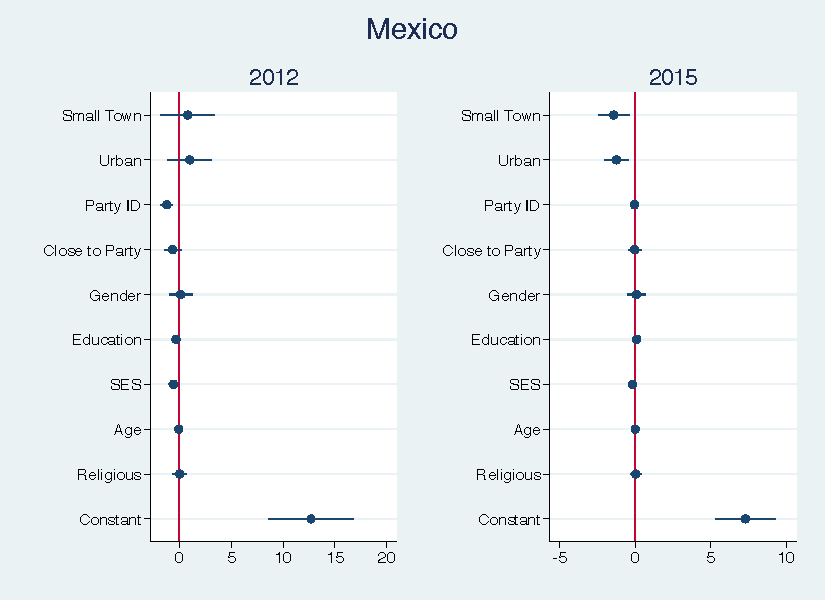
\includegraphics[width=\textwidth]{IdeologyCoef/Mexico}
	\end{subfigure}
	\hfill
	\begin{subfigure}[b]{0.475\textwidth}  
		\centering 
		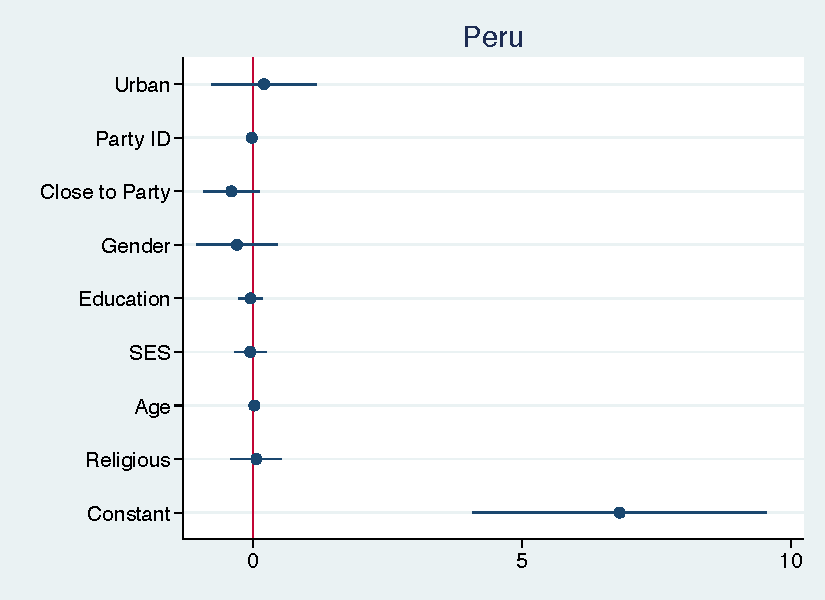
\includegraphics[width=\textwidth]{IdeologyCoef/Peru}
	\end{subfigure}
	\caption[ \tb{Self-Placement Ideology - Central/Latin America} ]
	{\tb {Coefficient Plots for Self-Placement Ideology in Central/Latin America} }
	\label{AmericaIdeo}
\end{figure}

Central America (as represented by Mexico in the 2012 and 2015 elections) and Latin American (represented by Peru) show some distinct patterns when it comes to the relationship of place and political ideology. Table \ref{table4} shows the results of the analysis. Both countries are relatively similar in their regime age, with Mexico being a democracy for 18 years at 2015 and Peru at 15 years in their 2016 election. Despite slightly different levels of democracy and distinct electoral formulas, both countries are relatively similar in their urban-rural trends. Both Mexico in 2012 and Peru show urban residents as more right leaning than their rural counterparts. Despite a relatively high coefficient, the difference is not statistically significant. However, Mexico in 2015 shows that urban residents are a point more to the left than their rural counterparts with statistical significance. This point difference is relatively large on a 10-point scale. For this region, we do not necessarily see regional similarities as only one polity (Mexico in 2015) supports the \e{Self-Identified Ideology} Hypothesis.

\begin{singlespace}
\begin{table}[H]
		\centering
		%\def\arraystretch{1.5}
		\caption{\tb{Self-Placement Ideology - Western Europe}}
		\begin{tabulary}{\linewidth}{l c c }

			\hline
			\tb{Place of Residence}&\tb{Germany}&\tb{France} \\
			\hline
			Small Town   & -.0753 &-.1266  \\      
			& (.2080)  & (.1680)   \\
			Suburban   & .2526 & -.0432    \\ 
			 & (.3290)  & (.2310)    \\
			Urban   & -.2544 & -.6460***    \\
			 &(.2490)  & (.1706)   \\
			Constant  & 5.399***  & 1.3237** \\
			&(0.0845)&(.6009) \\
			N  &427  & 1,332    \\
			$R^2$  &0.1072 &0.0866  \\
			\hline                                       
		\end{tabulary} 
		\\
		\e{Notes:} *p$<$.1, **p$<$.05. ***p$<$.01 \\
		\e{Reference:} A rural place of residence serves as the baseline for comparison
		\label{table5}
\end{table}
\end{singlespace}

\begin{figure}[H]
	\centering
	\begin{subfigure}[b]{0.475\textwidth}
		\centering
		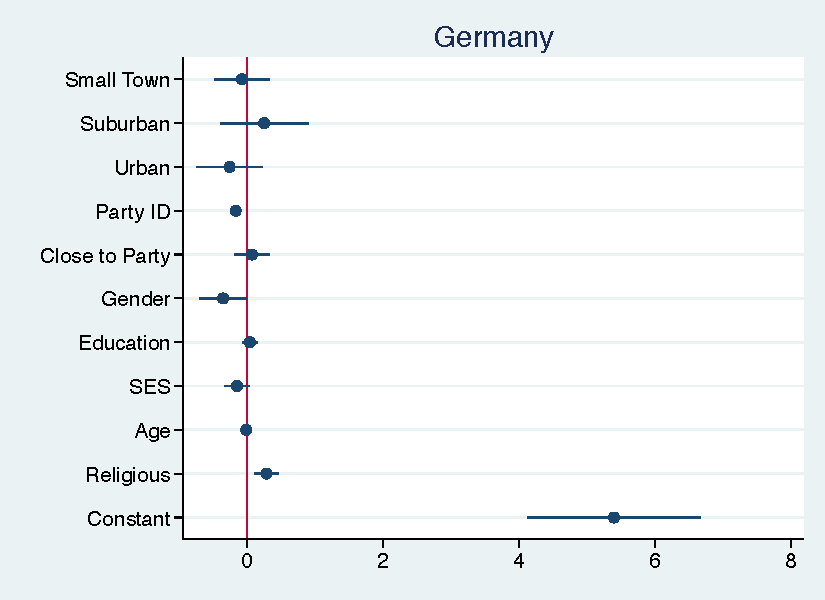
\includegraphics[width=\textwidth]{IdeologyCoef/Germany}
	\end{subfigure}
	\hfill
	\begin{subfigure}[b]{0.475\textwidth}  
		\centering 
		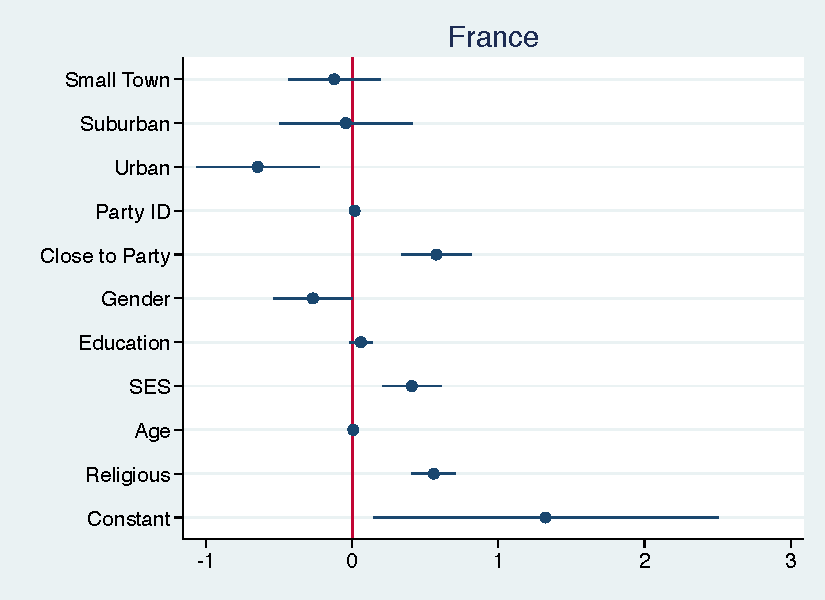
\includegraphics[width=\textwidth]{IdeologyCoef/France}
	\end{subfigure}
	\caption[ \tb{Self-Placement Ideology - Western Europe} ]
	{\tb {Coefficient Plots for Self-Placement Ideology in Western Europa} }
	\label{WestEuroIdeo}
\end{figure}

In Western Europe, the results confirm the \e{Self-Identified Ideology} hypothesis for France, but not Germany. In Table \ref{table5}, we can see that differences between France and Germany lie in the distinction between urban residents compared to rural residents. While both countries see urban residents lean left on the self-identified scale, France is more statistically significant in their .64 point jump to the left, which is relatively large for a 10 point scale. Geographically, Germany is considered more in Central Europe; however, their political activity makes them a worthwhile comparison to Western Europe.

\begin{singlespace}
	\begin{table}[H]
		\centering
		%\def\arraystretch{1.5}
		\caption{\tb{Self-Placement Ideology - Central Europe}}
		\begin{tabulary}{\linewidth}{l c c c c}

			\hline
			\tb{Place of Residence} &\tb{Austria}&\tb{Czech Republic}& \tb{Poland} &\tb{Slovakia} \\
			\hline
			Small Town&.6270**& -.1272 & .3032 & .3954  \\
			&(.3139) & (.2920) & (.2002) & (.3216) \\
			Suburban&-.0326& -.4467&.0666 & 2.1723\\
			&(.3343)&(.4993) & (.3104) & (.1.107)\\
			Urban&.3822&.5199 & .0954 & 1.1440 \\
			&(.3888) &(.2944) & (.2662) & (.4518) \\
			Constant& 4.014***& 3.930***& 5.096*** & 4.3473***  \\
			&(.9272) & (.8696) & (.8646) & (1.127) \\
			N&247& 511& 895 & 392 \\
			$R^2$&0.1126&0.2538 & 0.1348 & 0.1498 \\
			\hline
		\end{tabulary}
		\\
		\e{Notes:} *p$<$.1, **p$<$.05. ***p$<$.01 \\
		\e{Reference:} A rural place of residence serves as the baseline for comparison
		\label{table6}
	\end{table}
\end{singlespace}

\begin{figure}[H]
	\centering
	\begin{subfigure}[b]{0.475\textwidth}
		\centering
		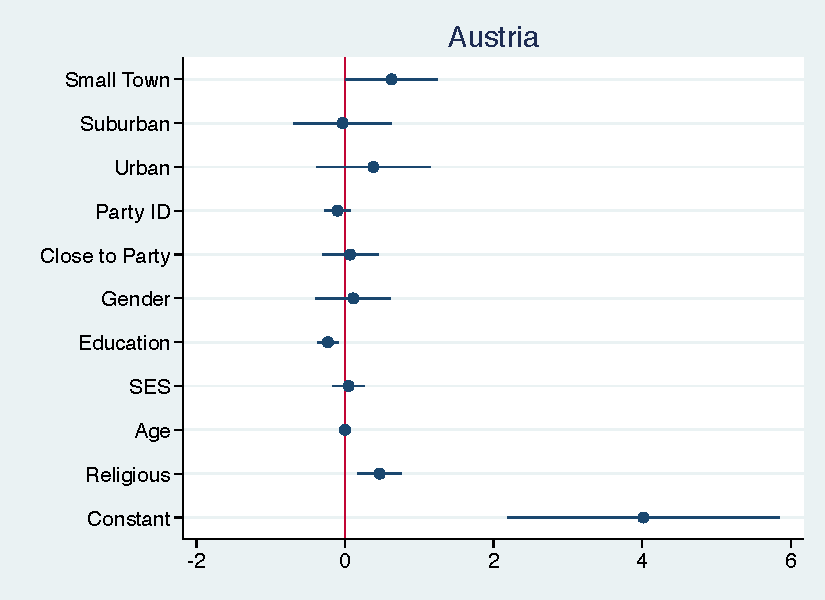
\includegraphics[width=\textwidth]{IdeologyCoef/Austria}
	\end{subfigure}
	\hfill
	\begin{subfigure}[b]{0.475\textwidth}  
	\centering 
		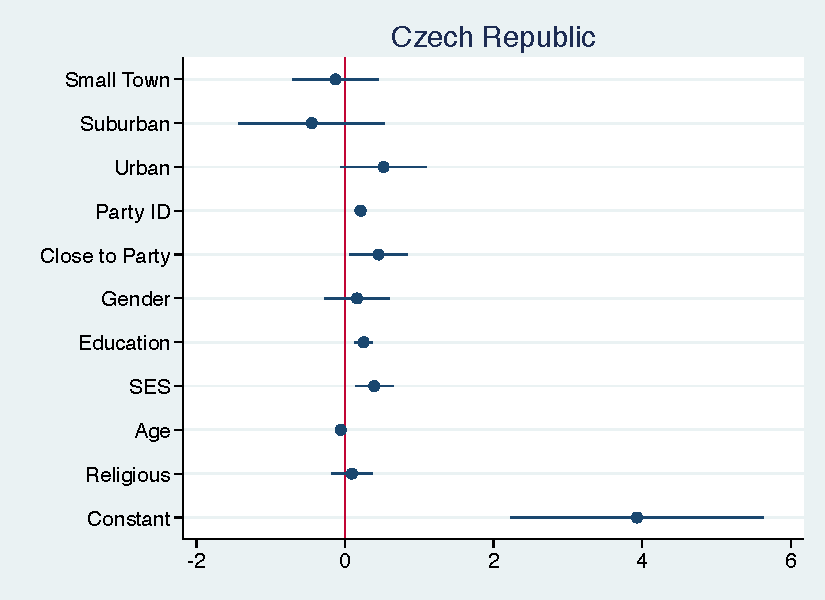
\includegraphics[width=\textwidth]{IdeologyCoef/Czech}
	\end{subfigure}
	\vskip\baselineskip
	\begin{subfigure}[b]{0.475\textwidth}   
		\centering 
		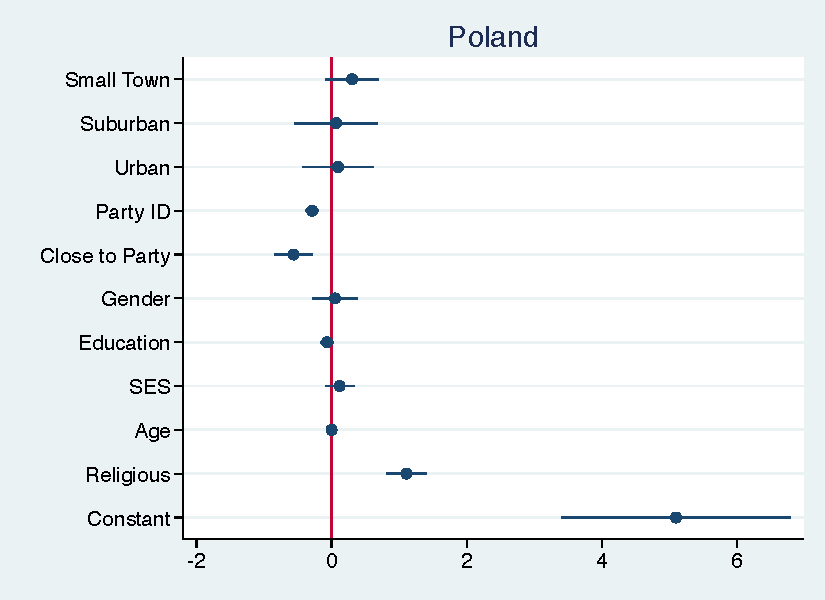
\includegraphics[width=\textwidth]{IdeologyCoef/Poland}
	\end{subfigure}
	\quad
	\begin{subfigure}[b]{0.475\textwidth}   
		\centering 
		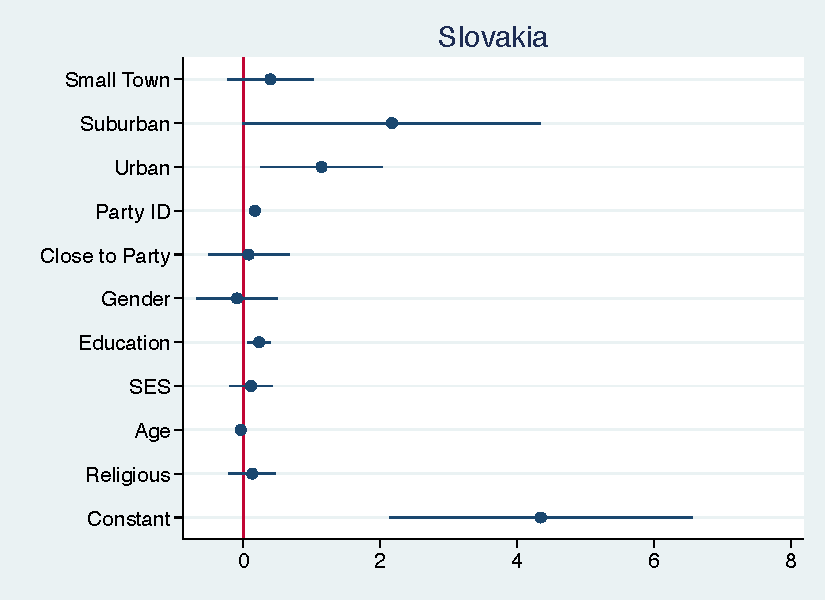
\includegraphics[width=\textwidth]{IdeologyCoef/Slovakia}
	\end{subfigure}
	\caption[ \tb{Self-Placement Ideology - Central Europe} ]
	{\tb {Coefficient Plots for Self-Placement Ideology in Central Europe} }
	\label{CentEuroIdeo}
\end{figure}


However, when placed in the context of the Central European states, Germany does fit in well with Austria, Czech Republic, Poland and Slovakia in terms of the rural-urban divide. All countries in this region are roughly 20-24 years of age, with a median of 23 years. Here, the regimes are all relatively free in terms of their level of democracy. With the exception of Germany, all regimes here are proportional systems. None of these countries show statistical significance when it comes to political ideologies in the form of self-identification. While many of the values are relatively large, there are good chances that these observations can be from chance alone. 

\begin{singlespace}
	\begin{table}[H]
		\centering
		%\def\arraystretch{1.5}
		\caption{\tb{Self-Placement Ideology - Scandinavia}}
		\begin{tabulary}{\linewidth}{l c c c}

			\hline
			\tb{Place of Residence}&\tb{Finland}&\tb{Iceland}&\tb{Sweden} \\
			\hline
			Small Town&.2546&1.131***&-.0247 \\
			&(.4143)&(.4036)&(.4636) \\
			Suburban&.0600&1.866***&.0325 \\
			&(.3463)&(.4081)&(.4431) \\
			Urban&-.6608&.9035**& .0217\\
			&(.4514)&(.3993)&(.4006) \\
			Constant&6.5998***&6.063***&2.352** \\
			&(1.123)&(.8182)&(1.116) \\
			N&187&428&330\\
			$R^2$&0.2158&0.1688&0.0677 \\
			\hline
		\end{tabulary}
		\\
		\e{Notes:} *p$<$.1, **p$<$.05. ***p$<$.01 \\
		\e{Reference:} A rural place of residence serves as the baseline for comparison
		\label{table7}
	\end{table}
\end{singlespace}

\begin{figure}[H]
	\centering
	\begin{subfigure}[b]{0.475\textwidth}
		\centering
		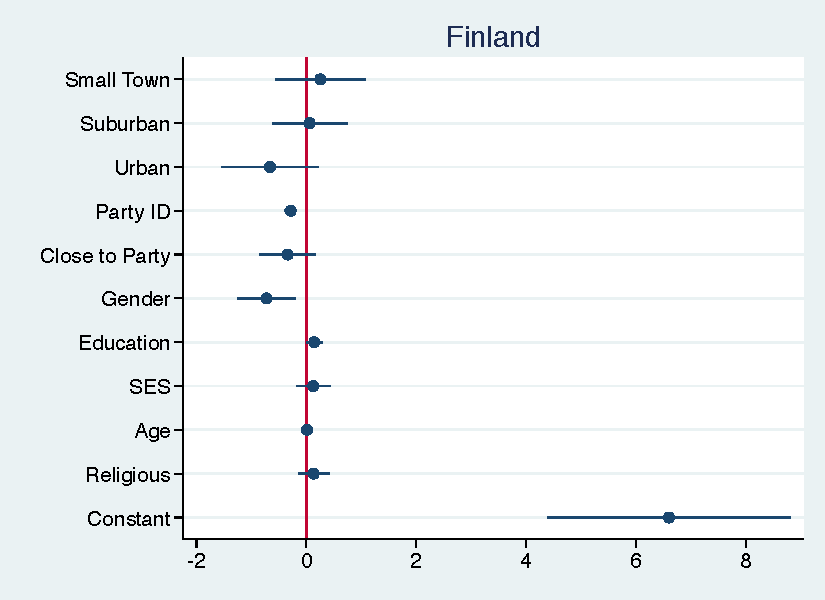
\includegraphics[width=\textwidth]{IdeologyCoef/Finland}
	\end{subfigure}
	\hfill
	\begin{subfigure}[b]{0.475\textwidth}  
		\centering 
		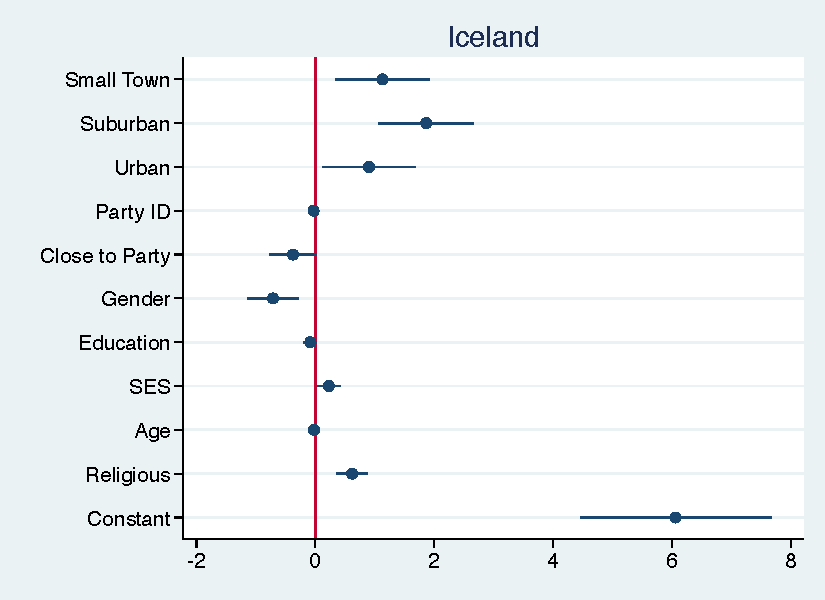
\includegraphics[width=\textwidth]{IdeologyCoef/Iceland}
	\end{subfigure}
	\vskip\baselineskip
	\begin{subfigure}[b]{0.475\textwidth}   
		\centering 
		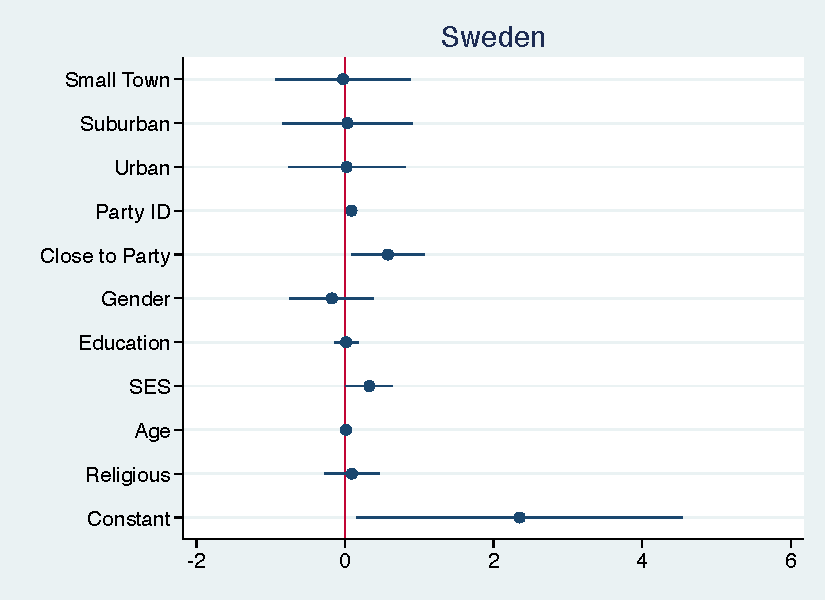
\includegraphics[width=\textwidth]{IdeologyCoef/Sweden}
	\end{subfigure}
	\caption[ \tb{Self-Placement Ideology - Scandinavia} ]
	{\tb {Coefficient Plots for Self-Placement Ideology in Scandinavia} }
	\label{ScandinaviaIdeo}
\end{figure}


Looking to the north, countries in the Scandinavian region are said to be some of the most free in Europe and also have relatively old democracies. As shown in Table \ref{table7}, the only country that shows significance in the urban-rural divide is Iceland, but it is nearly a full point to the right. Despite the statistical significance, this proves to be an interesting deviation from the \e{Self-Identified Ideology} hypothesis.

\begin{landscape}
	\begin{table}
		\centering
		\def\arraystretch{1.5}
		\caption{\tb{Self-Placement Ideology - Southwestern Europe}}
		\begin{tabulary}{\linewidth}{l c c c c c c}

			\hline
			\tb{Residence}& \tb{Bulgaria}& \tb{Greece ('12)}& \tb{Greece ('15)} & \tb{Montenegro} & \tb{Romania ('12)} & \tb {Romania ('14)}\\
			\hline
			Small Town&.2627 &-.0542 &-.3076 & -1.3042** & .0309 & .0511\\
			&(.3319)& (.5039) & (.4971) & (.5882) & (.3619) & (.6030)\\
			Suburban& .3400 & -.8706 &-.3540 & -.2289  &.2880 &.7052\\
			& (.2941) &(.4878) & (.5298) & (.8432) & (.8747) & (.7604)\\
			Urban& -.2833& -.8586** & -.3762 & .1149& 1.1965** & -.9908\\
			& (.4204)& (.3852) & (.4642) & (1.1020) & (.3769) & (.8057)\\
			Constant& 11.310*** &3.7549*** & 2.2395*** &7.633*** & 5.1379*** & 6.262***\\
			& (.9980) & (1.2241)  & (.9403) & (2.1586)& (1.3297) & (2.300)\\
			N& 440 & 360 & 476 & 152 & 566 &245\\
			$R^2$&0.5188 &0.1740& 0.1346 &0.1939& 0.0313 &0.1064 \\
			\hline
		\end{tabulary}
		\\
		\e{Notes:} *p$<$.1, **p$<$.05. ***p$<$.01 \\
		\e{Reference:} A rural place of residence serves as the baseline for comparison
		\label{table8}
	\end{table}
\end{landscape}

\begin{figure}[H]
	\centering
	\begin{subfigure}[b]{0.475\textwidth}
		\centering
		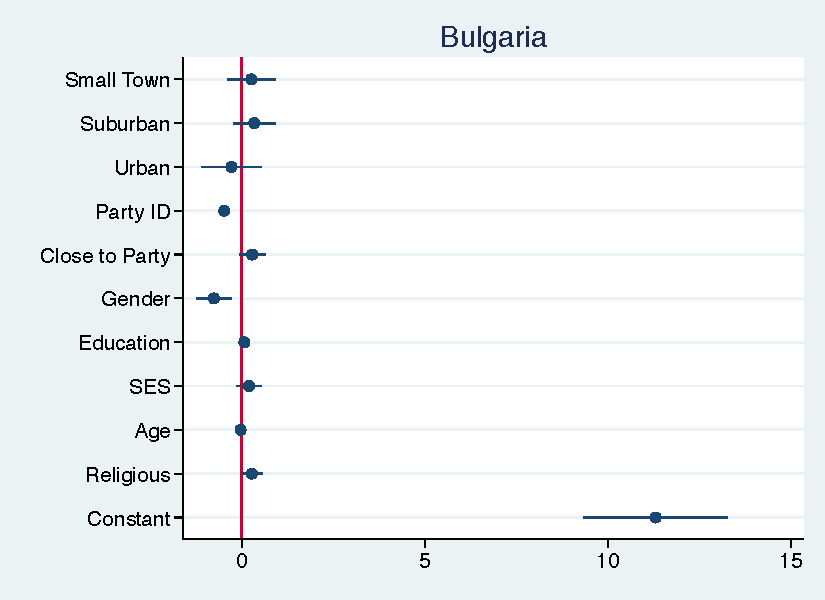
\includegraphics[width=\textwidth]{IdeologyCoef/Bulgaria}
	\end{subfigure}
	\hfill
	\begin{subfigure}[b]{0.475\textwidth}  
		\centering 
		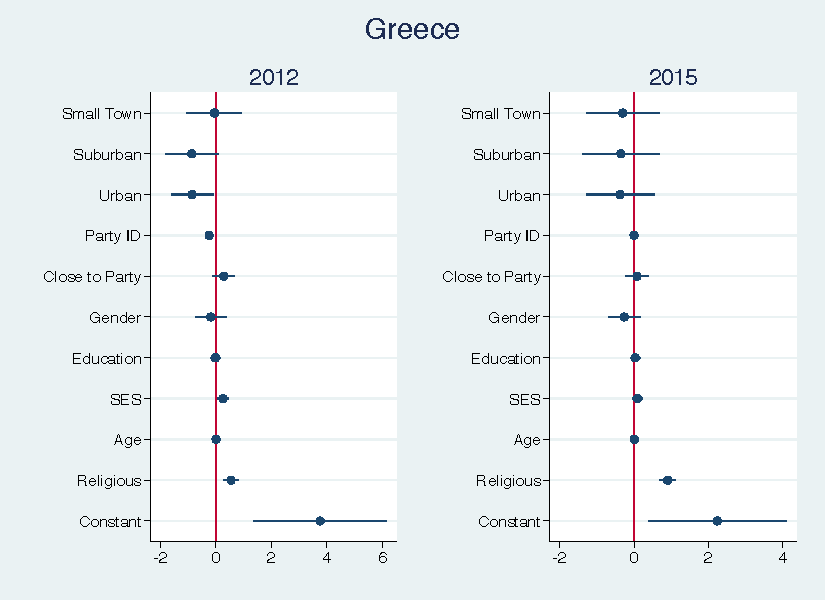
\includegraphics[width=\textwidth]{IdeologyCoef/Greece}
	\end{subfigure}
	\vskip\baselineskip
	\begin{subfigure}[b]{0.475\textwidth}   
		\centering 
		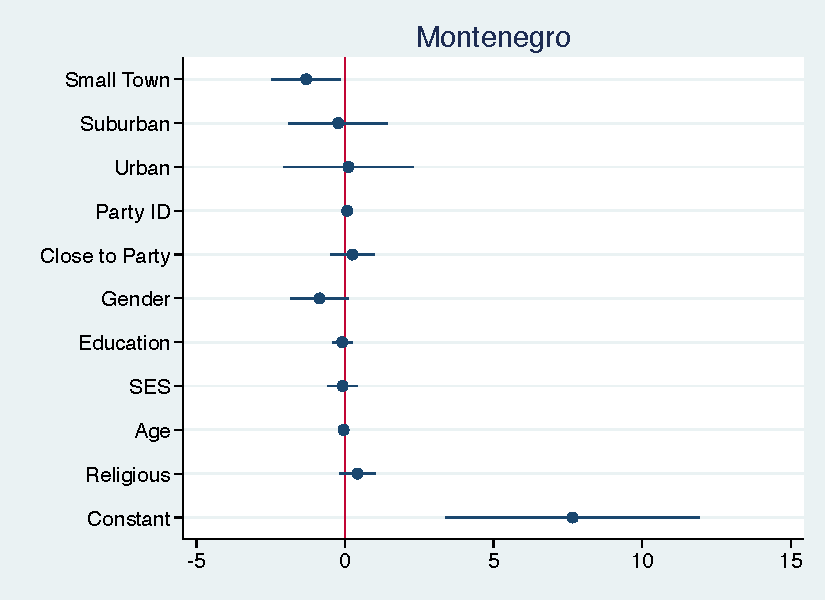
\includegraphics[width=\textwidth]{IdeologyCoef/Montenegro}
	\end{subfigure}
	\quad
	\begin{subfigure}[b]{0.475\textwidth}   
		\centering 
		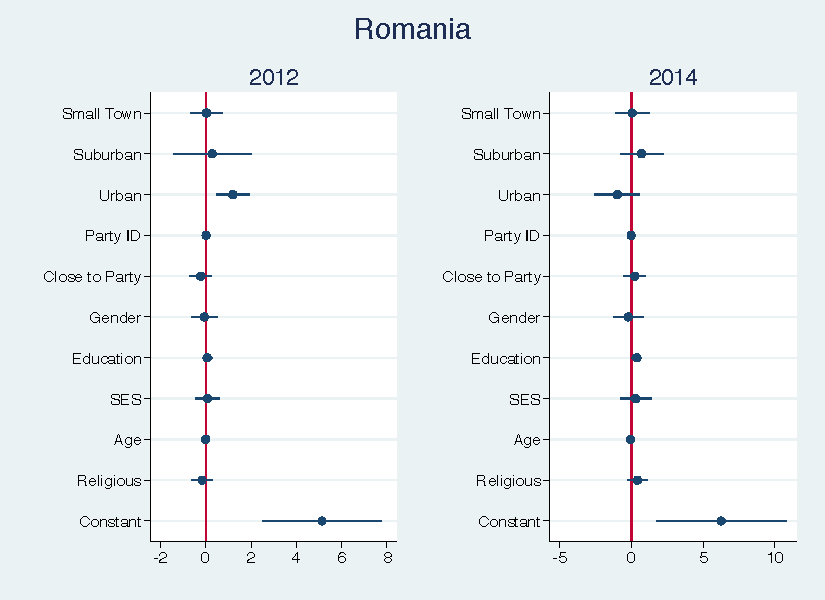
\includegraphics[width=\textwidth]{IdeologyCoef/Romania}
	\end{subfigure}
	\caption[ \tb{Self-Placement Ideology - Southwestern Europe} ]
	{\tb {Coefficient Plots for Self-Placement Ideology in Southwestern Europe} }
	\label{SWEuroIdeo}
\end{figure}

In Southwestern Europe, the results in Table \ref{table8} suggest an interesting set of results. For both Greece and Romania, the countries are represented by two elections and both are in a position where the former election suggests significance in place but not the latter. In Greece, the 2012 election respondents are more likely to lean left when living in an urban place of residence, which supports the \e{Self-Identified Ideology} hypothesis. However, this pattern is the opposite in Romania, where the 2012 respondents showed that urban residence led to more right-leaning political ideologies. The effect of place is not statistically significant in any other country in this region.

\begin{singlespace}
	\begin{table}[H]
		\centering
		%\def\arraystretch{1.5}
		\caption{\tb{Self-Placement Ideology - Eastern Europe}}
		\begin{tabulary}{\linewidth}{l c c}

			\hline
			\tb{Place of Residence} & \tb{Latvia (2011)} &\tb{Latvia (2014)} \\
			\hline
			Small Town &.0423 &-.1924 \\
			&(.5399) & (.4346) \\
			Suburban&- & -.1413 \\
			& - & (.5755) \\
			Urban&-.3829&-.3400 \\
			& (.4270) & (.3978) \\
			Constant & 5.502*** &7.8918*** \\
			& (1.4972) & (1.146) \\
			N&188 & 276\\
			$R^2$& 0.1469 &0.0424 \\
			\hline
		\end{tabulary}
		\\
		\e{Notes:} *p$<$.1, **p$<$.05. ***p$<$.01 \\
		\e{Reference:} A rural place of residence serves as the baseline for comparison
		\label{table9}
	\end{table}
\end{singlespace}

\begin{figure}[H]    \centering
	{	 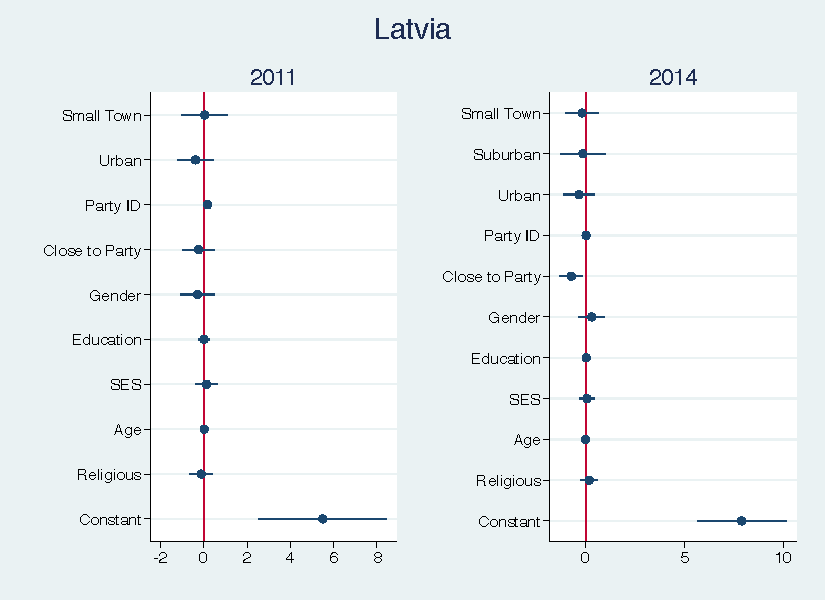
\includegraphics[width=.5\textwidth]{IdeologyCoef/Latvia}}
	\caption[ \tb{Self-Placement Ideology - Eastern Europe} ]
{\tb {Coefficient Plots for Self-Placement Ideology in Eastern Europe} }
\label{EastEuroIdeo}
\end{figure}

In Eastern Europe, Table \ref{table9} shows the results for Latvia's 2011 and 2014 elections and the results do not reflect patterns of influence with regards to place and ideology. With the consideration of the regime age, level of democracy and electoral formula, Latvia shares similar trends with states in Central and Southwestern Europe, which suggests that these macro-trends may play a role in explaining macro trends in the relationship between place of residence and an individual's political ideology. 

\begin{singlespace}
	\begin{table}[H]
		\centering
		%\def\arraystretch{1.5}
		\caption{\tb{Self-Placement Ideology - Middle East}}
		\begin{tabulary}{\linewidth}{l c c}

			\hline
			\tb{Place of Residence}&\tb{Israel} & \tb{Turkey} \\
			\hline
			Small Town&.5796 & .4447 \\
			&(.3041)  & (.6314)\\
			Suburban&.5968 &.3318 \\
			& (.3478)  & (.6740)\\
			Urban &- & .4440\\
			&- & (.5626)\\
			Constant& 6.1311*** &1.953 \\
			& (.9217)  & (1.813)\\
			N&439 & 251\\
			$R^2$&0.2978 & 0.1484 \\
			\hline 
		\end{tabulary}
		\\
		\e{Notes:} *p$<$.1, **p$<$.05. ***p$<$.01 \\
		\e{Reference:} A rural place of residence serves as the baseline for comparison
		\label{table10}
	\end{table}
\end{singlespace}

\begin{figure}[H]
	\centering
	\begin{subfigure}[b]{0.475\textwidth}
		\centering
		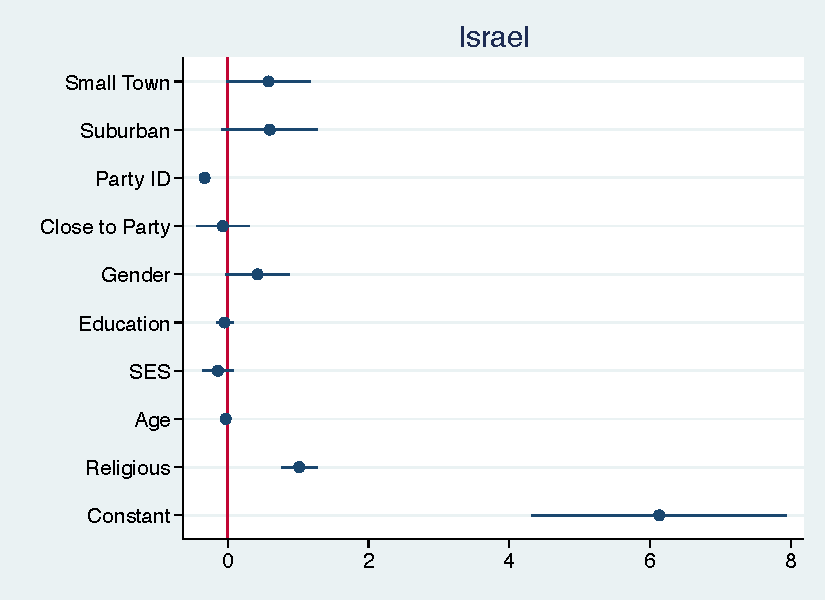
\includegraphics[width=\textwidth]{IdeologyCoef/Israel}
	\end{subfigure}
	\hfill
	\begin{subfigure}[b]{0.475\textwidth}  
		\centering 
		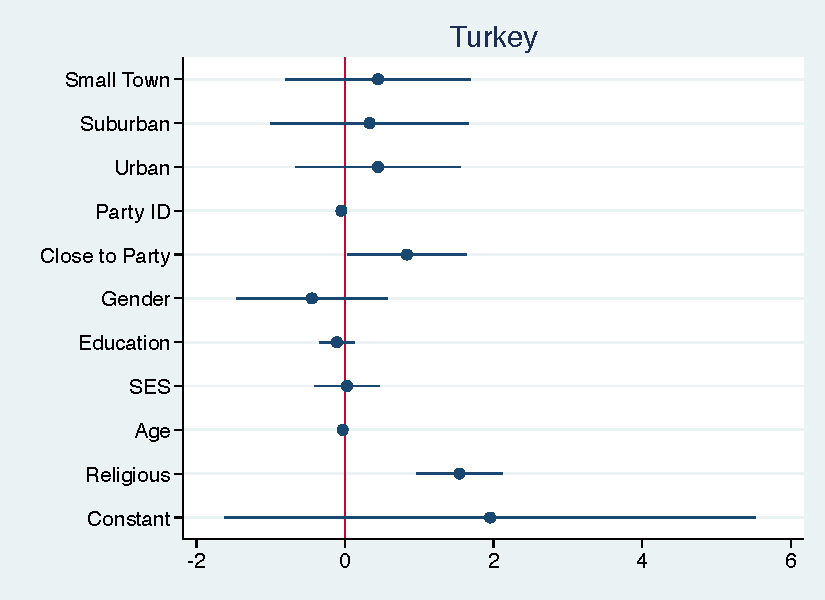
\includegraphics[width=\textwidth]{IdeologyCoef/Turkey}
	\end{subfigure}
	\caption[ \tb{Self-Placement Ideology - Middle East} ]
	{\tb {Coefficient Plots for Self-Placement Ideology in Middle East} }
	\label{MidEastIdeo}
\end{figure}

The Middle East provides an interesting set of countries since it exemplifies the one of the most free (Israel) and least free (Turkey) countries represented in this CSES dataset. These countries are both proportional in its electoral formula but differ by regime age. Yet, despite these differences, both countries do not show a place divide in political ideology. While Israel does not have an "urban center" due to the way place is defined in Israel, there are no signs of differences between any of the other areas and the rural settlements of the state.

\begin{singlespace}
	\begin{table}[H]
		\centering
		%\def\arraystretch{1.5}
		\caption{\tb{Self-Placement Ideology - Africa}}
		\begin{tabulary}{\linewidth}{l c}

			\hline
			\tb{Place of Residence}& \tb{South Africa} \\
			\hline
			Urban&-1.0519** \\
			&(.4499)\\
			Constant&8.7909*** \\
			& (1.5955) \\
			N& 220\\
			$R^2$&0.0660 \\
			\hline
		\end{tabulary}
		\\
		\e{Notes:} *p$<$.1, **p$<$.05. ***p$<$.01 \\
		\e{Reference:} A rural place of residence serves as the baseline for comparison
		\label{table11}
	\end{table}
\end{singlespace}

\begin{figure}[H]    \centering
	{	 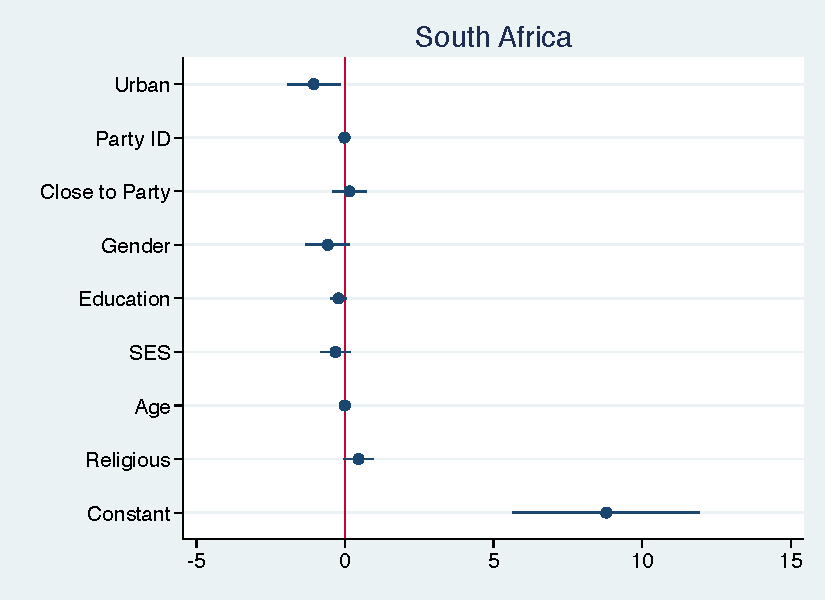
\includegraphics[width=.5\textwidth]{IdeologyCoef/SouthAfrica}}
	\caption[ \tb{Self-Placement Ideology - Africa} ]
	{\tb {Coefficient Plots for Self-Placement Ideology in Africa} }
	\label{AfricaIdeo}
\end{figure}

Africa was originally represented by both Kenya and South Africa. However, with the introduction of controls, the lack of response in one of the areas led to the isolation of South Africa as the sole state in Africa for this analysis. The continent of Africa is one of the most recent places to transition to democracy in the wake of the decolonization movements. However, despite being a democracy for only 20 years, South Africa shows that there are differences between their urban and rural residents with their urban residents rating themselves a full point to the left. It is important to note that place of residence was not directly asked of the participants during the data collection. It is a code used by the researchers for identification purposes. Nonetheless, the results in Table \ref{table11} suggest that there is a significant difference between residents in rural and urban places in a recently transitioned regime in Africa, a trend that is not seen in their Central and Eastern European counterparts that share a regime age and level of democracy.

\begin{singlespace}
	\begin{table}[H]
		\centering 
		%\def\arraystretch{1.5}
		\caption{\tb{Self-Placement Ideology - Asia}}
		\begin{tabulary}{\linewidth}{l c c}

			\hline
			\tb{Place of Residence} & \tb{Japan} & \tb{South Korea}\\
			\hline
			Small Town &.6578** & -.5849 \\
			&(.2648) & (.4634)\\
			Suburban&.5867** & -2.233*** \\
			& (.2796) & (.7757)\\
			Urban & .6344** &.0059 \\
			& (.2576) & (4217)\\
			Constant& 6.0168*** & .4540 \\
			& (.7272) & (1.495)\\
			N&528 & 267\\
			$R^2$&0.0886 & 0.2113\\
			\hline
		\end{tabulary}
		\\
		\e{Notes:} *p$<$.1, **p$<$.05. ***p$<$.01 \\
		\e{Reference:} A rural place of residence serves as the baseline for comparison
		\label{table12}
	\end{table}
\end{singlespace}

\begin{figure}[H]
	\centering
	\begin{subfigure}[b]{0.475\textwidth}
		\centering
		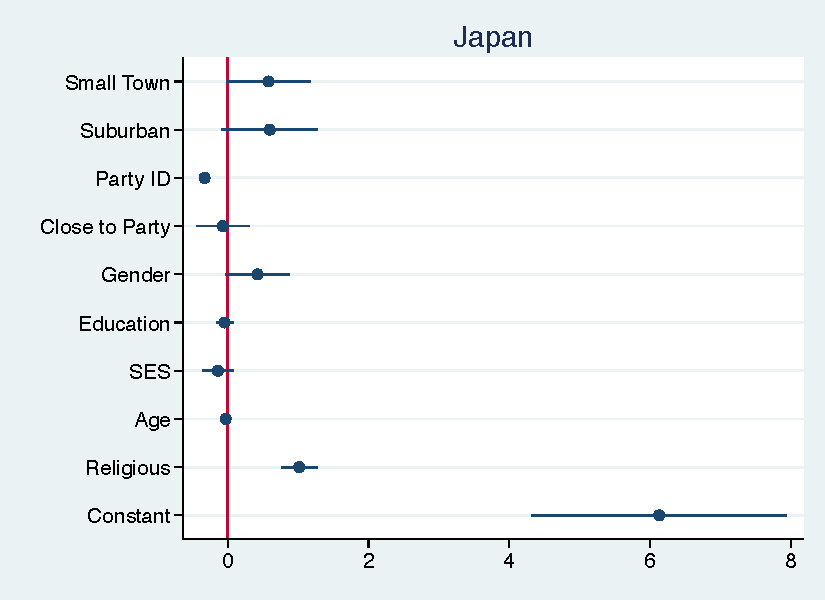
\includegraphics[width=\textwidth]{IdeologyCoef/Japan}
	\end{subfigure}
	\hfill
	\begin{subfigure}[b]{0.475\textwidth}  
		\centering 
		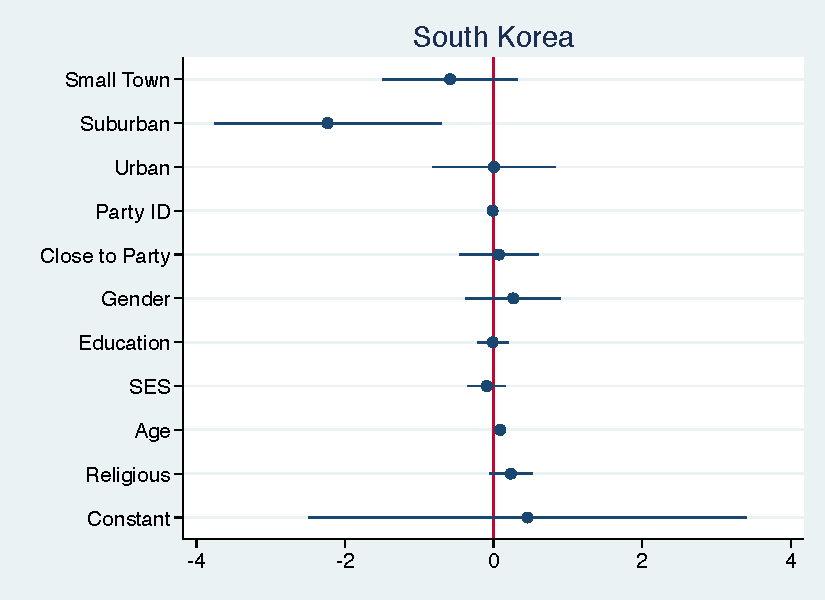
\includegraphics[width=\textwidth]{IdeologyCoef/SouthKorea}
	\end{subfigure}
	\caption[ \tb{Self-Placement Ideology - Asia} ]
	{\tb {Coefficient Plots for Self-Placement Ideology in Asia} }
	\label{AsiaIdeo}
\end{figure}

Table \ref{table12} show the patterns in Asia represented by Japan and South Korea. Both countries utilize the mixed electoral formula. Japan is older than South Korea as a regime and also more free. Respondents to the Japan study showed difference in place of residence when it comes to political ideology. The residents of Japan's urban centers (cities more than 200,000 people) tend to be more conservative by close to two-thirds of a point on the 10-point ideology scale. The move to the right is gradually seen through the responses of the small town and suburban residents of Japan as well. In South Korea, suburban residents are two and a quarter points to the left of their rural counterparts, suggesting that the \e{Self-Identified Ideology} phenomena happens in the suburbs of South Korea than in the urban centers. 

By geography, the Philippines are often considered to be part of Asia given the ethnic identities of the people; however, their geographic location can also qualify them to be a pacific island. Therefore, while Table \ref{table13} shows the trends of the Philippines and New Zealand, I will analyze them in the broader context of Asia. The Philippines is a relatively young democracy and has a rating of 8 on the level of democracy scale. New Zealand has one of the most free in the region (similar to Japan) and is also the oldest. Yet, none of these two countries show a place divide when it comes to political ideology. Therefore, in Asia as a whole, the presence of a rural-urban divide in some countries and not others suggest that there is not a regional influence not are there patterns between levels of democracy, regime age, and electoral formula that influence the relationship between place of residence and political ideology.

\begin{singlespace}
	\begin{table}[H]
		\centering
		%\def\arraystretch{1.5}
		\caption{\tb{Self-Placement Ideology - Pacific Islands}}
		\begin{tabulary}{\linewidth}{l c c }

			\hline
			\tb{Place of Residence}&\tb{New Zealand (2011)}&\tb{Philippines}\\
			\hline
			Small Town & -.3603  & .6010  \\      
			& (.3050) & (.8141)    \\
			Suburban  & -   & .7878  \\ 
			 & -   & (1.4391)       \\
			Urban  & -.0154   & .3447 \\
			 &(.2926)   & (.4770)      \\
			Constant  & 5.176***  & 7.838***   \\
			&(.8503)&(1.8952) \\
			N  &586 & 115  \\
			$R^2$  &0.0491  &0.0627     \\
			\hline                                       
		\end{tabulary} 
		\\
		\e{Notes:} *p$<$.1, **p$<$.05. ***p$<$.01 \\
		\e{Reference:} A rural place of residence serves as the baseline for comparison
		\label{table13}
	\end{table}
\end{singlespace}

\begin{figure}[H]
	\centering
	\begin{subfigure}[b]{0.475\textwidth}
		\centering
		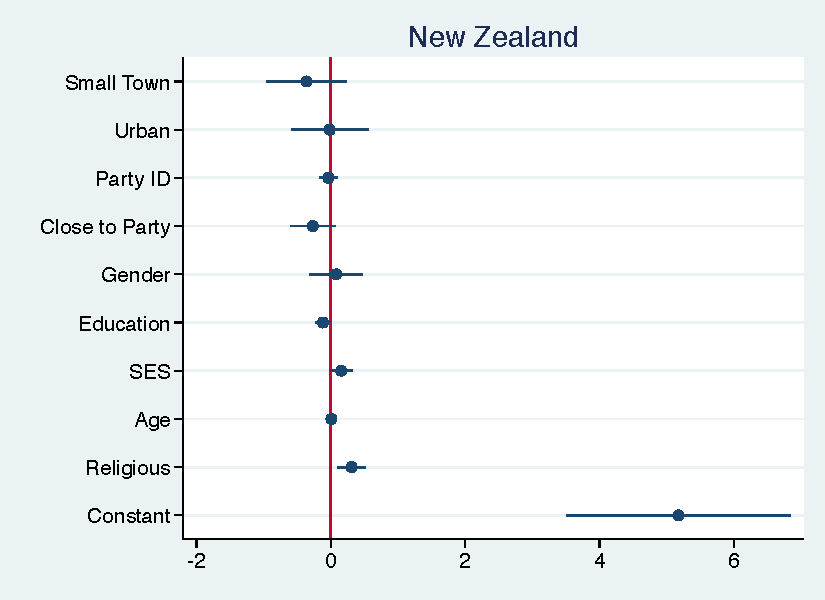
\includegraphics[width=\textwidth]{IdeologyCoef/NewZealand}
	\end{subfigure}
	\hfill
	\begin{subfigure}[b]{0.475\textwidth}  
		\centering 
		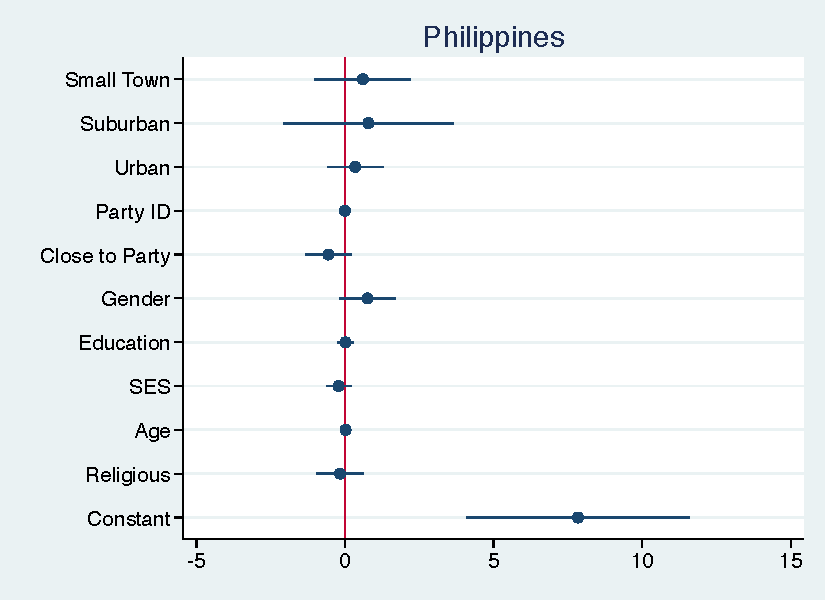
\includegraphics[width=\textwidth]{IdeologyCoef/Philippines}
	\end{subfigure}
	\caption[ \tb{Self-Placement Ideology - Pacific Islands} ]
	{\tb {Coefficient Plots for Self-Placement Ideology in Pacific Island} }
	\label{PacificIdeo}
\end{figure}

\subsubsection{Summary: Place Matters?}

Throughout this analysis of regions and considerations of specific polities' political idiosyncrasies, we cannot discern a pattern that shows how place of residence influences how one places themselves on the ideological spectrum, nor can we discern a pattern from how macro variables such as regime age, level of democracy and electoral formula influences the effects that the variables have on each other. Additionally, with the exception of Central and Eastern Europe, there does not seem to be another region where the countries that are represented in this dataset have some form of discernible regional pattern.

In the next section, I turn to the influence of place using an objective measure of beliefs in political actions based on social and economic policy and spending. From here, we can see if there is a relationship between how individuals describe themselves and how their objective issue stances play out based on where they live.

\subsection{Objective Issue Stances as a Dependent Measure}

In the previous section, I looked at specific countries to try to discern the extent to which place matters in a person's self placement on the political ideology spectrum. From the results of that model, we can see that place matters, but the country to which the place is embedded in also matters to determine and influence the relationship between the variables. In this section, I aim to explore a more objective variable on liberalism to see the extent to which place really matters in influencing individual political attitudes towards economic and social inequality. As previous research suggests (notably, \cite{walsh_putting_2012}), residents of rural environments tend to be more conservative when it comes to social spending, even if the results will work in their favor. 

The analysis employed in this section will look at general trends to see if there is indeed an influence between place and positions on spending. A variable was created for this analysis which aggregates the views that people have for spending government money on various social services in the country (see Appendix \ref{AppendixB} for more information on variable coding). 

%Fixed to include Controls
\begin{table}[h!]
	\centering
	%\def\arraystretch{1.5}
	\caption{\tb{Issue Stances - General Trends}}
	\begin{tabulary}{\linewidth}{l c}

		\hline
		\tb{Place of Residence} & \tb{Worldwide} \\
		\hline 
		Small Town&.0432 \\
		&(.0278)\\
		Suburban&.0082\\
		&(.0352) \\
		Urban&.0995*** \\
		&(.0272)\\
		Constant&2.7915*** \\
		&(.0762) \\
		N&9.662 \\
		$R^2$&0.0195 \\
		\hline
	\end{tabulary}
	\\
\e{Notes:} *p$<$.1, **p$<$.05. ***p$<$.01 \\
\e{Reference:} A rural place of residence serves as the baseline for comparison
\label{table14}
\end{table}

\begin{figure}[H]    \centering
	{	 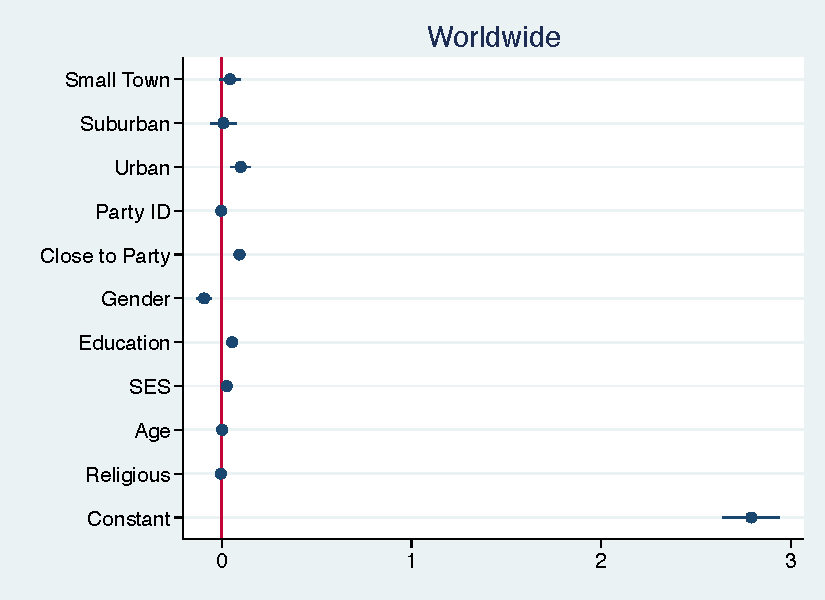
\includegraphics[width=.8\textwidth]{CoefAlllib}}
	\caption{\tb{Coefficient Plot for Global Issue Stances Trends}}\label{WorldIdeoLib}
\end{figure}

From the results that reflects general trends in the world based on the new liberalism variable, we see that there are some differences between place of residence and issue stances. Looking at Table \ref{table14} alongside the earlier Table \ref{table3}, we see that there urban-rural divide is less pronounced than it was before. (Both Tables are reproduced in Appendix \ref{AppendixD} for simplicity in comparison). The results here parallel the findings in the self-placement ideology analyses. Here, on a worldwide scale, respondents who live in an urban area are more likely to lean conservative but the tilt towards conservatism is not as great of a point jump compared to the self-placement ideology as a dependent variable. This suggests that people may, on average, place themselves farther to the right or left, but this feeling of placement on the spectrum is not entirely reflected in the way they truly view the issues.


\subsubsection{Consideration of Issue Stances by Geographic Region}

Now, we proceed to break down this general analysis by the same regions used to test the \e{Self-Identified Ideology} Hypothesis. 

\begin{singlespace}
	\begin{table}[H]
		\centering
		%\def\arraystretch{1.5}
		\caption{\tb{Issue Stances - Central/Latin America}}
		\begin{tabulary}{\linewidth}{l c c c}
			
			\hline
			\tb{Place of Residence}&\tb{Mexico (2012)}&\tb{Mexico (2015)} &\tb{Peru}\\
			\hline
			Small Town&-.2407 & .3685*& - \\
			&(.4166)  & (.2180)&-\\
			Suburban&- &- &-\\
			& -  & -&-\\
			Urban &-.0589 & .1503&-.014\\
			&(.3661) & (.1577)&(.1250)\\
			Constant& 2.8517*** &3.6772***&2.760*** \\
			& (..6696)  & (.4178&(.3451)\\
			N&110 & 335&262\\
			$R^2$&0.0575 & 0.0321&0.0589 \\
			\hline 
		\end{tabulary}
		\\
		\e{Notes:} *p$<$.1, **p$<$.05. ***p$<$.01 \\
		\e{Reference:} A rural place of residence serves as the baseline for comparison
		\label{CentAmerLib}
	\end{table}
\end{singlespace}

\begin{figure}[H]
	\centering
	\begin{subfigure}[b]{0.475\textwidth}
		\centering
		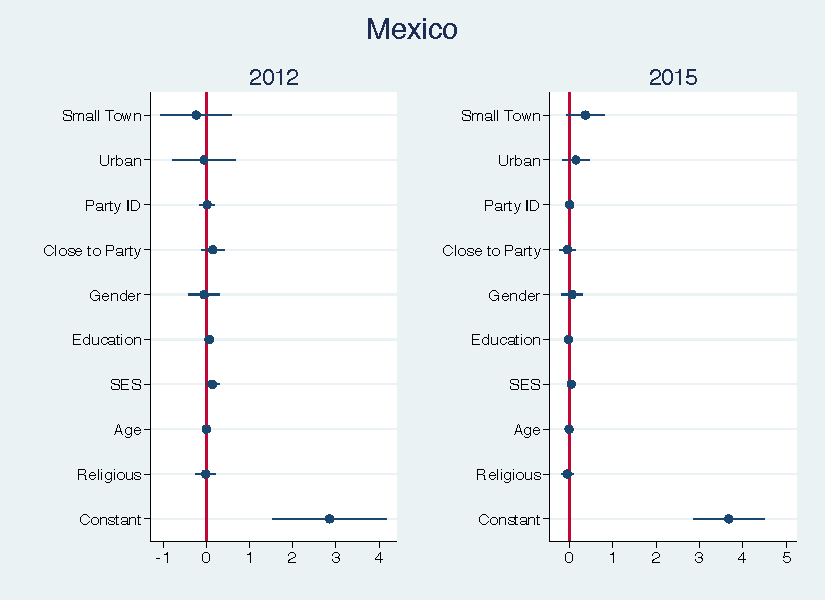
\includegraphics[width=\textwidth]{LibCoef/Mexico}
	\end{subfigure}
	\hfill
	\begin{subfigure}[b]{0.475\textwidth}  
		\centering 
		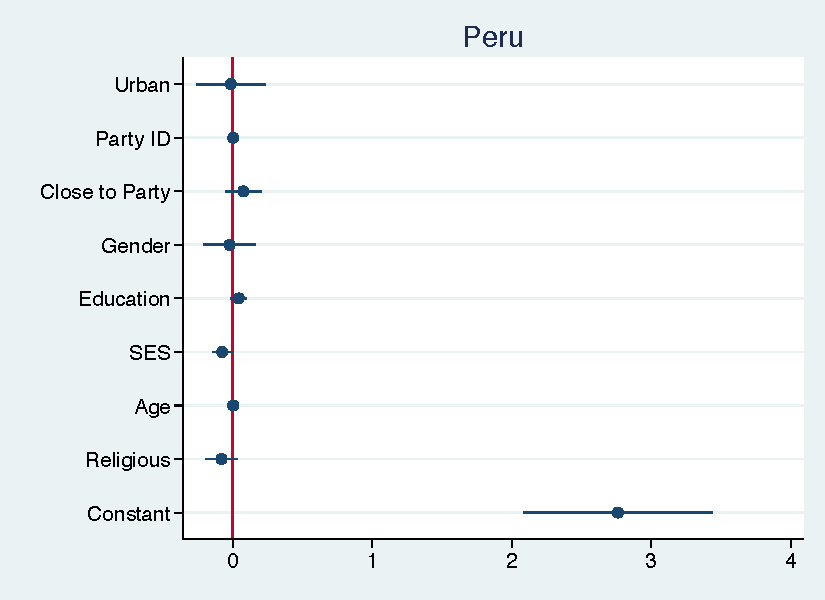
\includegraphics[width=\textwidth]{LibCoef/Peru}
	\end{subfigure}
	\caption[ \tb{Issue Stances - Central/Latin America} ]
	{\tb {Coefficient Plots for Issue Stances in Central/Latin America} }
	\label{AmericaLibCoef}
\end{figure}

In Central and Latin America, the results for the \e{Issue Stances} hypothesis for this region does not suggest a similar pattern as the \e{Self-Identified Ideology} results since none of the countries in this region show statistical significance when place of residence is regressed with the Issue Stances/Liberalism variable. For these results, it suggests that place of residence does not influence the ways the people view issues relating to government spending.

\begin{singlespace}
	\begin{table}[H]
		\centering
		%\def\arraystretch{1.5}
		\caption{\tb{Issue Stances - Western Europe}}
		\begin{tabulary}{\linewidth}{l c c }
		
			\hline
			\tb{Place of Residence}&\tb{Germany}&\tb{France} \\
			\hline
			Small Town& .0236 & -.0362   \\
			&(.1004)  & (.0648)\\
			Suburban&-.1950&-.1163 \\
			&(.1549) &  (.0926) \\
			Urban & .1514&.0188 \\
			&(.1195) &(.0846) \\
			Constant&2.920*** &2.001*** \\
			&(.3134) &(.2402) \\
			N&418& 1,159\\
			$R^2$&0.0873 & 0.0512 \\
			\hline 
\end{tabulary}
\\
\e{Notes:} *p$<$.1, **p$<$.05. ***p$<$.01 \\
\e{Reference:} A rural place of residence serves as the baseline for comparison
\label{WELib}
\end{table}
\end{singlespace}

\begin{figure}[H]
	\centering
	\begin{subfigure}[b]{0.475\textwidth}
		\centering
		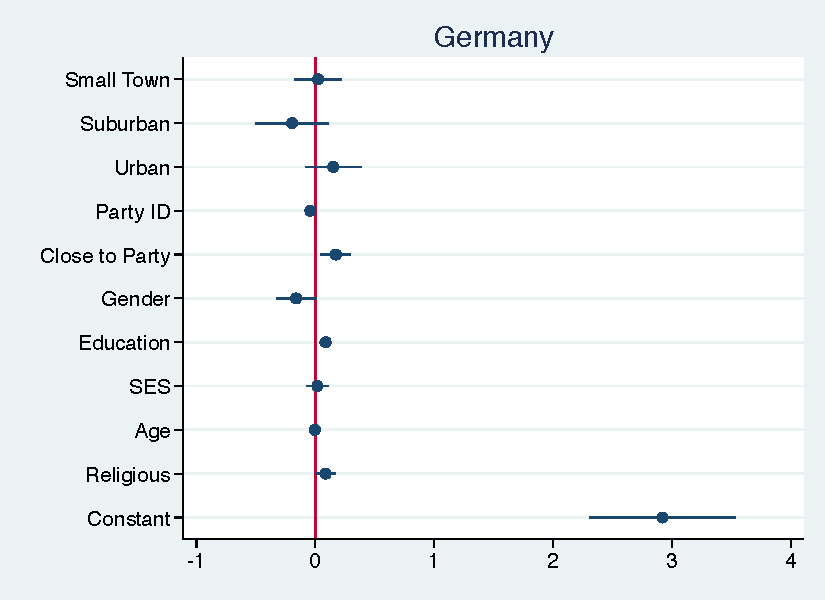
\includegraphics[width=\textwidth]{LibCoef/Germany}
	\end{subfigure}
	\hfill
	\begin{subfigure}[b]{0.475\textwidth}  
		\centering 
		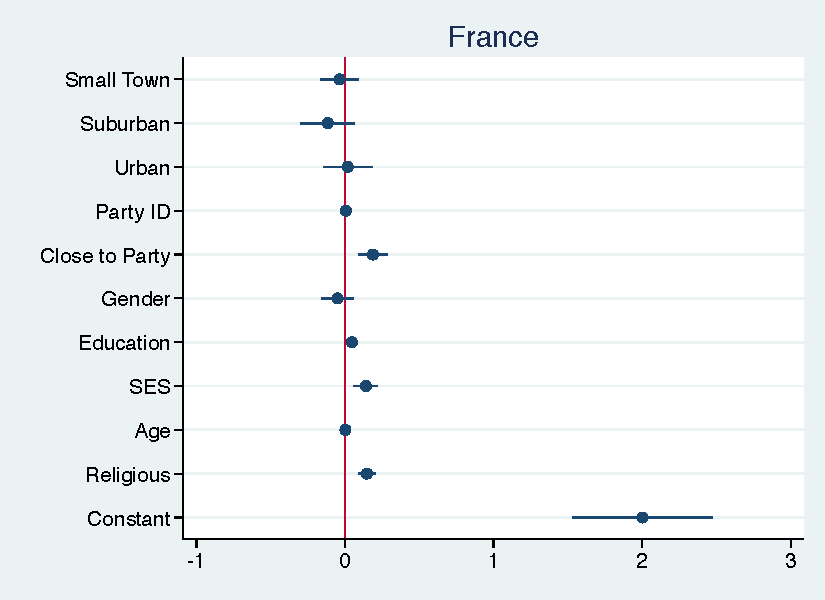
\includegraphics[width=\textwidth]{LibCoef/France}
	\end{subfigure}
	\caption[ \tb{Issue Stances - Western Europe} ]
	{\tb {Coefficient Plots for Issue Stances in Western Europa} }
	\label{WestEuroLib}
\end{figure}

When we turn to Western Europe, we see a similar trend that Central and Latin America has with the results between the two dependent variables. Under the \e{Self-Identified Ideology} hypothesis model, France's citizens showed that living in a more urban place led to greater feelings of left-leaning sentiment, but the general trends under the \e{Issue Stances} hypothesis model does not show this. Rather, there is a movement towards the right, albeit not as significant. These patterns are also seen in Central Europe. with the exception of Czech Republic. While the country moved towards the right in the previous model, there was no indication of a real difference between places of residence and political attitudes. However, their shift under the present model suggests that when it comes to objective issue stances, there is a difference between urban and rural residents. The suburban residents of Poland also show that place matters between rural villages and suburbia when is comes to attitudes towards government spending such that suburban residents are more liberal, but this effect is not seen in the urban centers.

Unlike the Self-Placement Ideology model, the results for the Issue Stances suggests that individuals in all of the Scandinavian countries do not differ drastically based on their attitudes towards government spending given place of residence differences. 

\begin{singlespace}
	\begin{table}[H]
		\centering
		%\def\arraystretch{1.5}
		\caption{\tb{Issue Stances - Central Europe}}
		\begin{tabulary}{\linewidth}{l c c c }
			
			\hline
			\tb{Place of Residence} &\tb{Austria}&\tb{Czech Republic}& \tb{Poland} \\
			\hline
			Small Town &.0045 &.1837  &-.0045   \\
			&(.1289)&(.1167) &(.0778)  \\
			Suburban& .0362 &.3035  &-.2401**   \\
			&(.1345) &(.1967) &(.1164)\\
			Urban&-.1473&.4128***  &-.0112    \\
			&(.1622)& (.1166)  &(.1008)    \\
			Constant&4.3364*** &3.3739***  &2.637***     \\
			N&246 & 448  & 711   \\
			$R^2$&0.0674&0.1258  &0.0546  \\
			\hline 
\end{tabulary}
\\
\e{Notes:} *p$<$.1, **p$<$.05. ***p$<$.01 \\
\e{Reference:} A rural place of residence serves as the baseline for comparison
\label{CELib}
\end{table}
\end{singlespace}

\begin{figure}[H]
	\centering
	\begin{subfigure}[b]{0.475\textwidth}
		\centering
		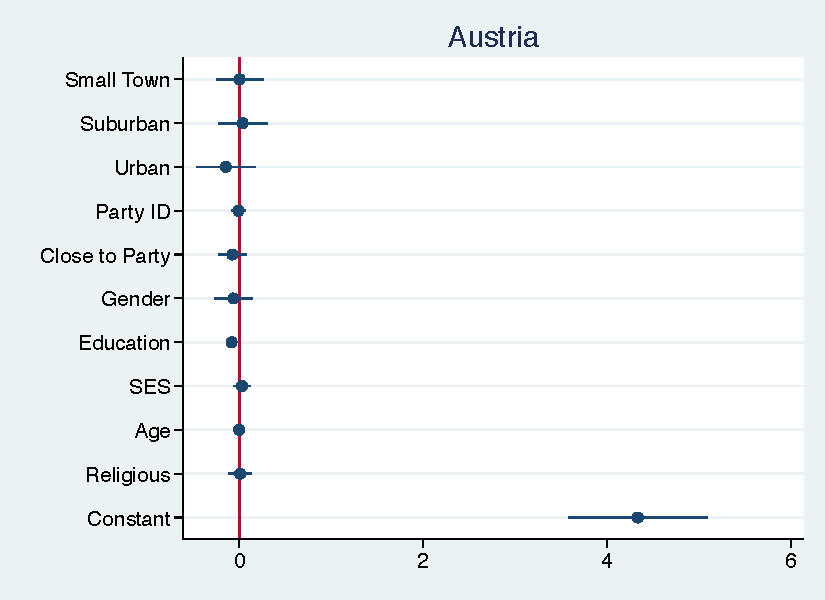
\includegraphics[width=\textwidth]{LibCoef/Austria}
	\end{subfigure}
	\hfill
	\begin{subfigure}[b]{0.475\textwidth}  
		\centering 
		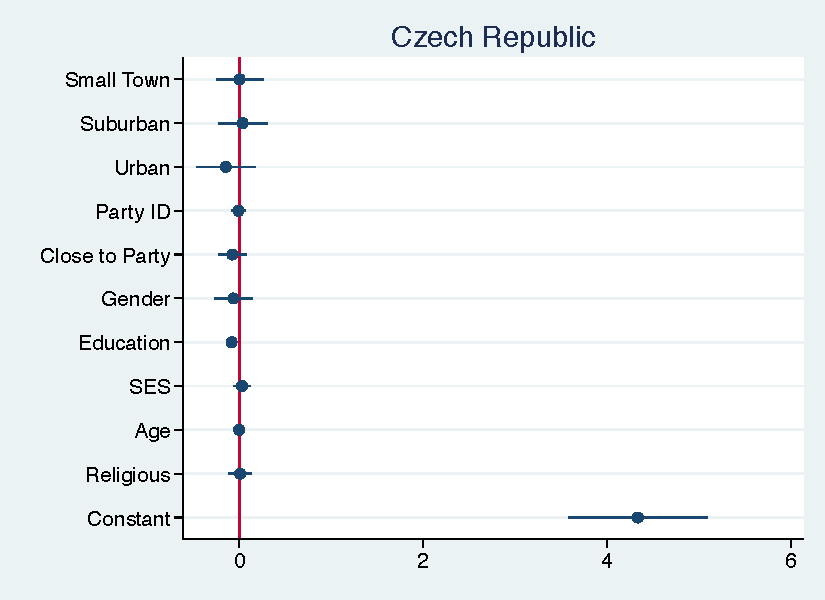
\includegraphics[width=\textwidth]{LibCoef/Czech}
	\end{subfigure}
	\vskip\baselineskip
	\begin{subfigure}[b]{0.475\textwidth}   
		\centering 
		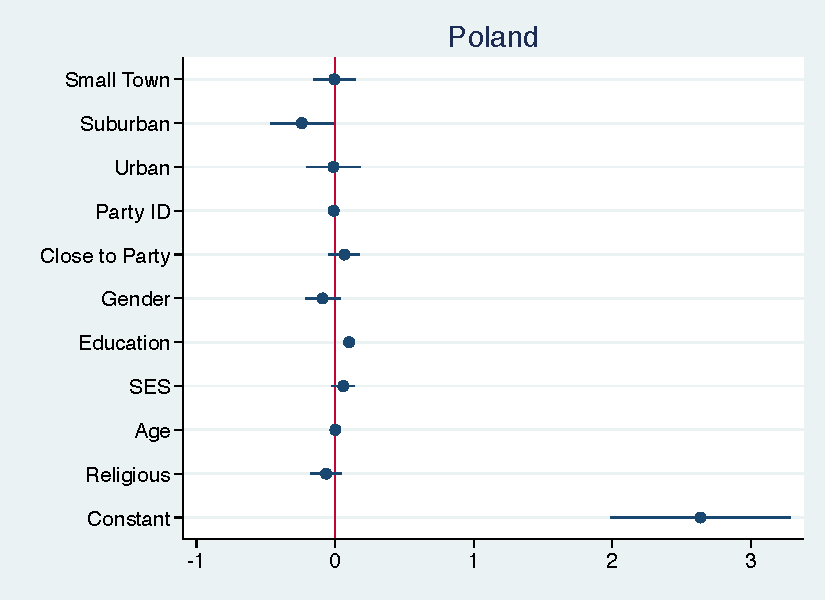
\includegraphics[width=\textwidth]{LibCoef/Poland}
	\end{subfigure}
	\caption[ \tb{Issue Stances - Central Europe} ]
	{\tb {Coefficient Plots for Issue Stances in Central Europe} }
	\label{CentEuroLibCoef}
\end{figure}


\begin{singlespace}
	\begin{table}[H]
		\centering
		%\def\arraystretch{1.5}
		\caption{\tb{Issue Stances - Scandinavia}}
		\begin{tabulary}{\linewidth}{l c c c}
			\hline
			\tb{Place of Residence}&\tb{Finland}&\tb{Iceland}&\tb{Sweden} \\
			\hline
			Small Town& -.0501 &.1522 & -.1209 \\
			&(.1997) & (.1830) & (.1828) \\
			Suburban&-.0150&.2700  &-.1410  \\
			&(.1651) &(.1852) & (.1745) \\
			Urban &.0677 &.1158  & -.0144 \\
			&(.2131) & (.1819) & (.1578) \\
			Constant&3.9752*** &3.995***  & 3.6204*** \\
			&(.5452) &(.3722) & (.4453) \\
			N&198&372 &284  \\
			$R^2$&0.1154&.1055  & 0.0362 \\  
			\hline
\end{tabulary}
\\
\e{Notes:} *p$<$.1, **p$<$.05. ***p$<$.01 \\
\e{Reference:} A rural place of residence serves as the baseline for comparison
\label{ScanLib}
\end{table}
\end{singlespace}

\begin{figure}[H]
	\centering
	\begin{subfigure}[b]{0.475\textwidth}
		\centering
		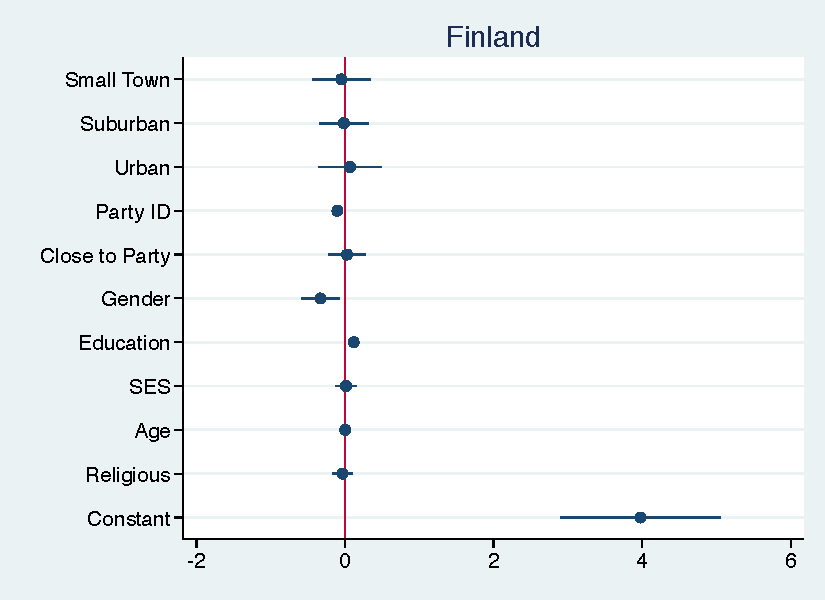
\includegraphics[width=\textwidth]{LibCoef/Finland}
	\end{subfigure}
	\hfill
	\begin{subfigure}[b]{0.475\textwidth}  
		\centering 
		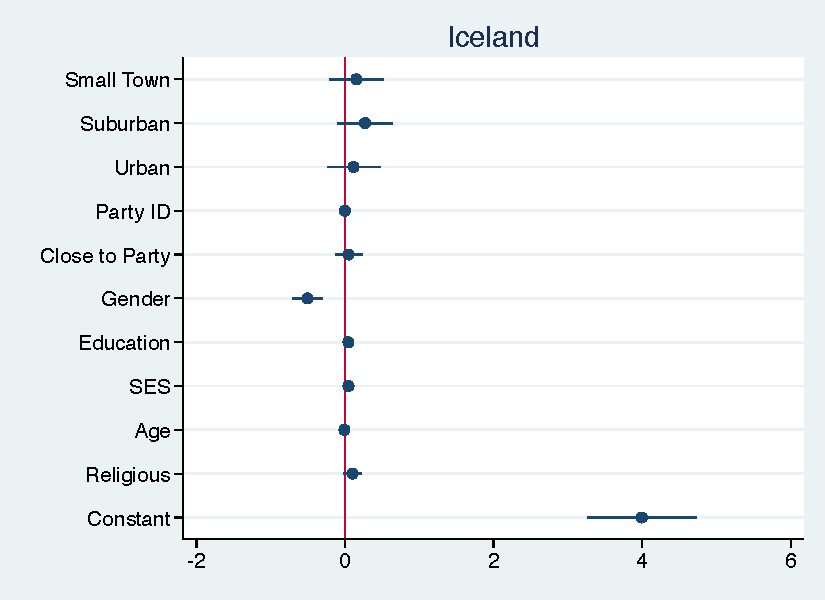
\includegraphics[width=\textwidth]{LibCoef/Iceland}
	\end{subfigure}
	\vskip\baselineskip
	\begin{subfigure}[b]{0.475\textwidth}   
		\centering 
		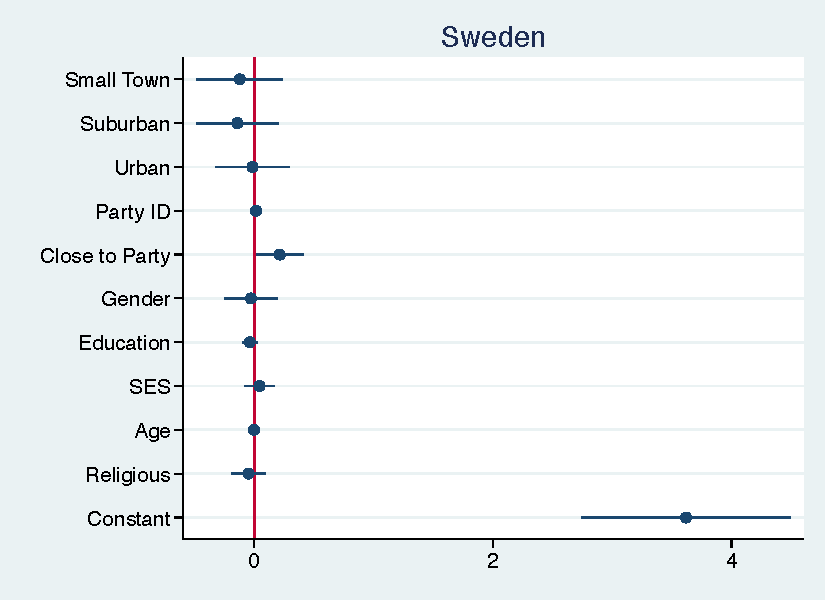
\includegraphics[width=\textwidth]{LibCoef/Sweden}
	\end{subfigure}
	\caption[ \tb{Issue Stances - Scandinavia} ]
	{\tb {Coefficient Plots for Issue Stances in Scandinavia} }
	\label{ScandinaviaLib}
\end{figure}

\begin{landscape}
	\begin{table}
		\centering
		\def\arraystretch{1.5}
		\caption{\tb{Issue Stances - Southwestern Europe}}
		\begin{tabulary}{\linewidth}{l c c c c c c}
			\hline
			\tb{Residence}& \tb{Bulgaria}& \tb{Greece ('12)}& \tb{Greece ('15)} & \tb{Montenegro} & \tb{Romania ('12)} & \tb {Romania ('14)}\\
			\hline
			Small Town& -.0295&-.3396 &-.3025 &.6388*** & -.0862 &.1283  \\
			&(.1228) &(.2166)  &(.2420)  & (.2069) & (.0838)  & (.1352)  \\
			Suburban& .3420***&-.4875** &-.3352  & .6956** & -.2285  & .0263 \\
			&(.1111)& (.2118)  &(.2598)  &(.3059)  & (.2096) & (.1698) \\
			Urban&.2230& -.4093** & -.3739*  & .6014* & .1614* &-.1373  \\
			&(.1663)& (.1729) &(.2263)   & (.3558)  & (.0839) & (.1817)  \\
			Constant&3.0603***&2.360***  & 2.598*** & 3.4274*** &2.6031***  & 3.4728***  \\
			&(.3741)& (.5231)  &(.4582)  &(.8088)  & (.2963) & (.5290)  \\
			N&391 & 329  &458   & 184 & 659  &263  \\
			$R^2$&0.0899& 0.1420  &0.0457  & 0.1014 & 0.0365 & 0.0414 \\
			\hline
\end{tabulary}
\\
\e{Notes:} *p$<$.1, **p$<$.05. ***p$<$.01 \\
\e{Reference:} A rural place of residence serves as the baseline for comparison
\label{SWELib}
\end{table}
\end{landscape}

\begin{figure}[H]
	\centering
	\begin{subfigure}[b]{0.475\textwidth}
		\centering
		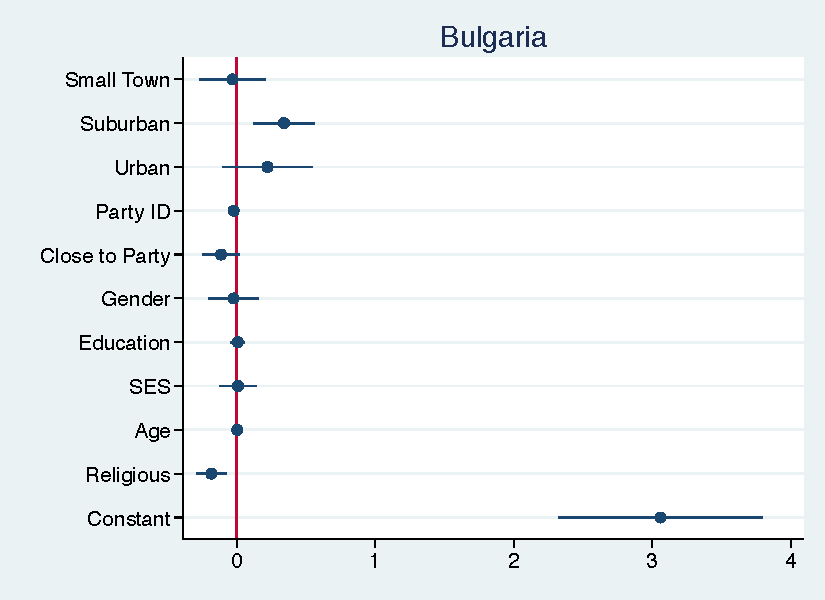
\includegraphics[width=\textwidth]{LibCoef/Bulgaria}
	\end{subfigure}
	\hfill
	\begin{subfigure}[b]{0.475\textwidth}  
		\centering 
		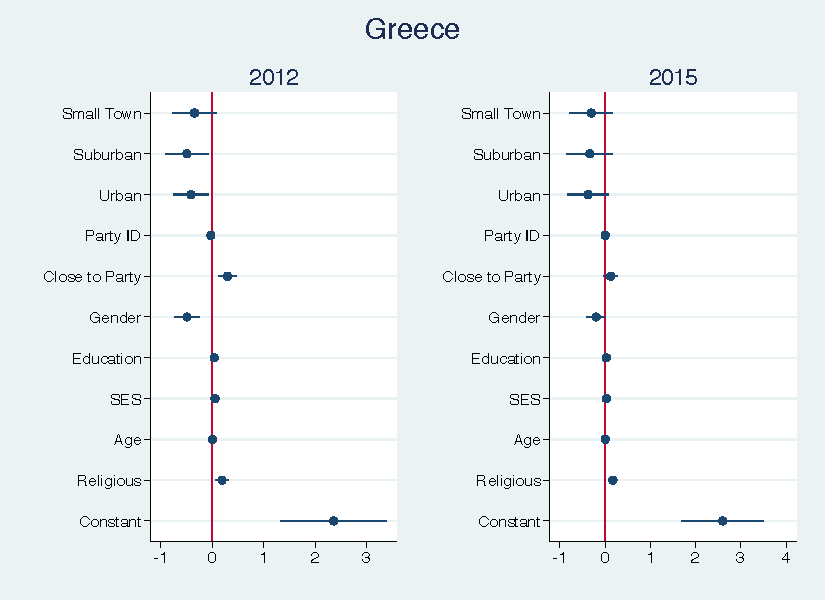
\includegraphics[width=\textwidth]{LibCoef/Greece}
	\end{subfigure}
	\vskip\baselineskip
	\begin{subfigure}[b]{0.475\textwidth}   
		\centering 
		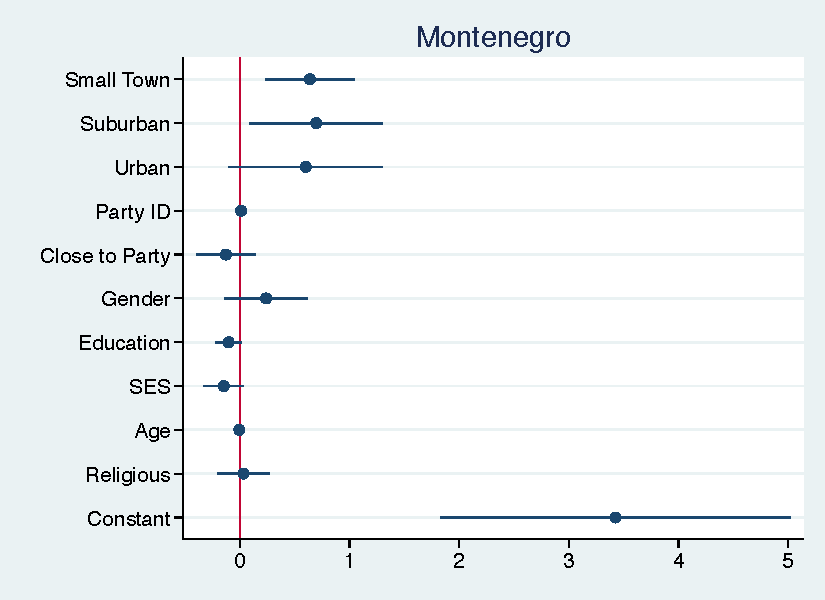
\includegraphics[width=\textwidth]{LibCoef/Montenegro}
	\end{subfigure}
	\quad
	\begin{subfigure}[b]{0.475\textwidth}   
		\centering 
		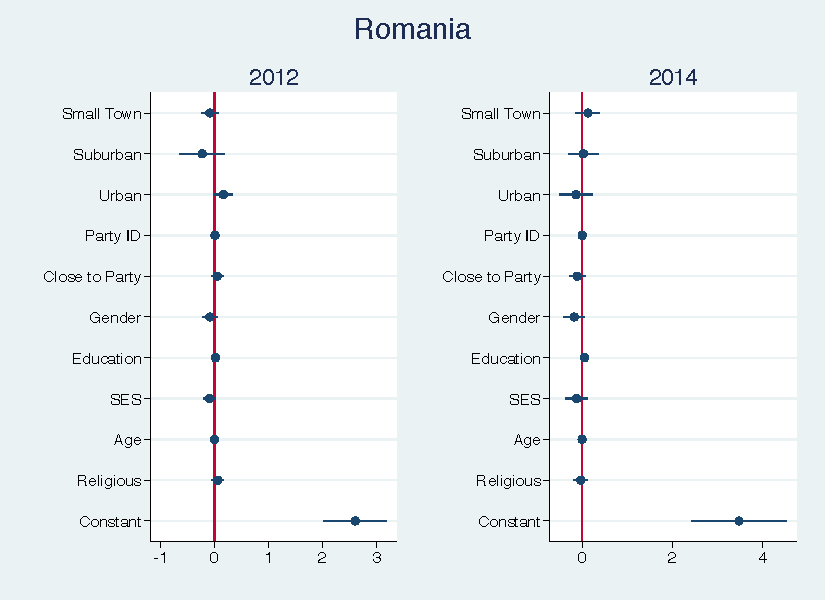
\includegraphics[width=\textwidth]{LibCoef/Romania}
	\end{subfigure}
	\caption[ \tb{Issue Stances - Southwestern Europe} ]
	{\tb {Coefficient Plots for Issue Stances in Southwestern Europe} }
	\label{SWEuro}
\end{figure}

In Southwestern Europe, Greece confirms the \e{Issue Stances} hypothesis such that the urban residents are more likely than chance to say that they are more open to government spending than rural residents. This pattern is observed in the opposite direction for Montenegro and Romania in 2012. Yet, the same cannot be said for Latvia in their 2014 election, the sole case here from Eastern Europe. 

\begin{singlespace}
	\begin{table}[H]
		\centering
		%\def\arraystretch{1.5}
		\caption{\tb{Issue Stances - Eastern Europe}}
		\begin{tabulary}{\linewidth}{l c }

			\hline
			\tb{Place of Residence} & \tb{Latvia (2014)}  \\
			\hline
			Small Town& -.4632*** \\
			&(.1475)\\
			Suburban&-.2366\\
			&(.2049)\\
			Urban&-.0163\\
			&(.1355)\\
			Constant&2.5914***\\
			&(.3932)\\
			N&276\\
			$R^2$&0.1014\\
			\hline
\end{tabulary}
\\
\e{Notes:} *p$<$.1, **p$<$.05. ***p$<$.01 \\
\e{Reference:} A rural place of residence serves as the baseline for comparison
\label{EastELib}
\end{table}
\end{singlespace}


\begin{figure}[H]    \centering
	{	 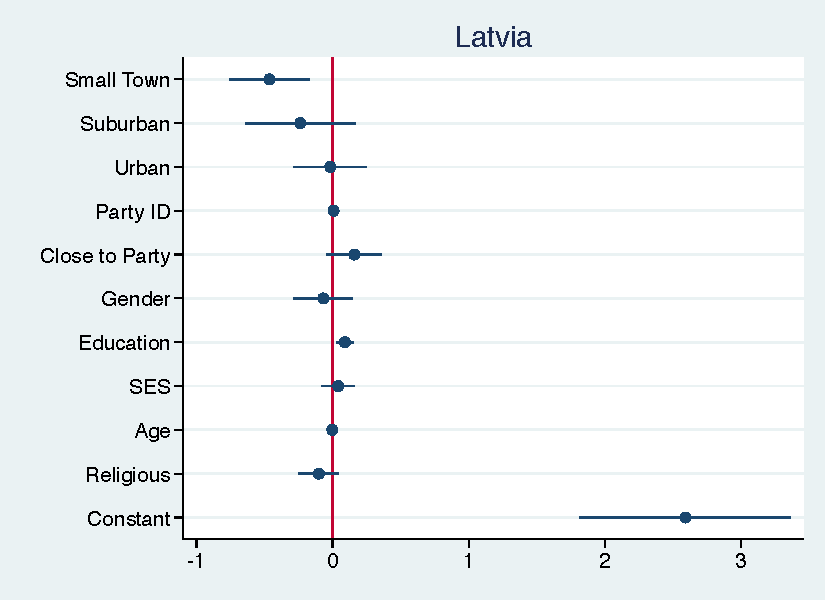
\includegraphics[width=.5\textwidth]{LibCoef/Latvia}}
	\caption[ \tb{Issue Stances - Eastern Europe} ]
	{\tb {Coefficient Plots for Issue Stances in Eastern Europe} }
	\label{EastEuroLibCoef}
\end{figure}


In the non-European parts of the world, no country shows statistically significant differences between place of residence and issue attitude differences except for Thailand and the Philippines. For Thailand, the data for self-identified ideology was unavailable, so there does not exist a base for comparison in our model. However, the results here suggest that urban residents are more likely to lean close to a full point to the right when it comes to issue stances regarding government spending. In the Philippines, the opposite is true as urban residents are more likely to favor government spending given that they lean over a half a point to the left on average. These results can be seen in Table \ref{AsiaLib} and Table \ref{PacificLib}.

\begin{singlespace}
	\begin{table}[H]
		\centering
		%\def\arraystretch{1.5}
		\caption{\tb{Issue Stances - Middle East}}
		\begin{tabulary}{\linewidth}{l c c}

			\hline
			\tb{Place of Residence}&\tb{Israel} & \tb{Turkey} \\
			\hline
			Small Town&.1159&-.1208 \\
			&(.1147)&(.2029) \\
			Suburban&.0637 &.2178 \\
			&(.1312) &(.2178) \\
			Urban&- &.1028 \\
			&- &(.1783)\\
			Constant&3.4492***&1.886*** \\
			&(.3445)&(.5757) \\
			N&379&252 \\
			$R^2$&0.0544&0.0875 \\
			\hline
\end{tabulary}
\\
\e{Notes:} *p$<$.1, **p$<$.05. ***p$<$.01 \\
\e{Reference:} A rural place of residence serves as the baseline for comparison
\label{MELib}
\end{table}
\end{singlespace}

\begin{figure}[H]
	\centering
	\begin{subfigure}[b]{0.475\textwidth}
		\centering
		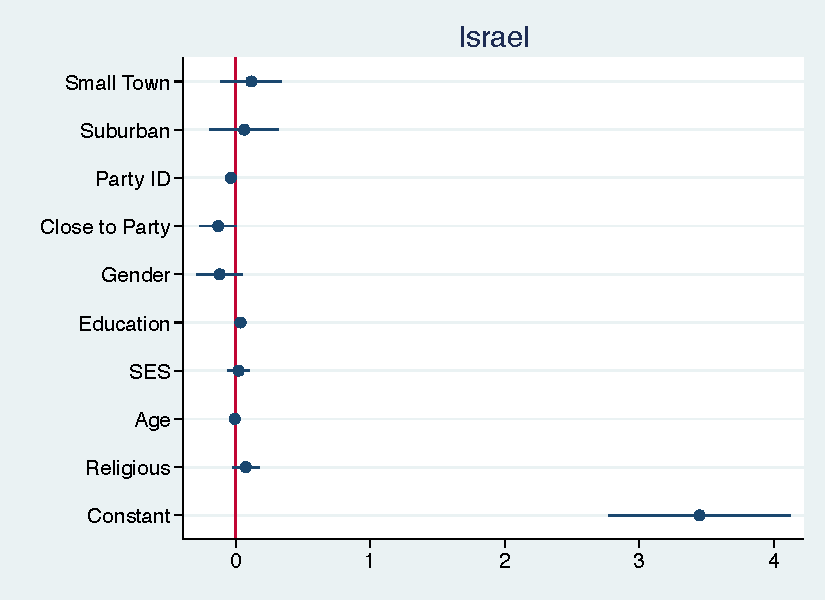
\includegraphics[width=\textwidth]{LibCoef/Israel}
	\end{subfigure}
	\hfill
	\begin{subfigure}[b]{0.475\textwidth}  
		\centering 
		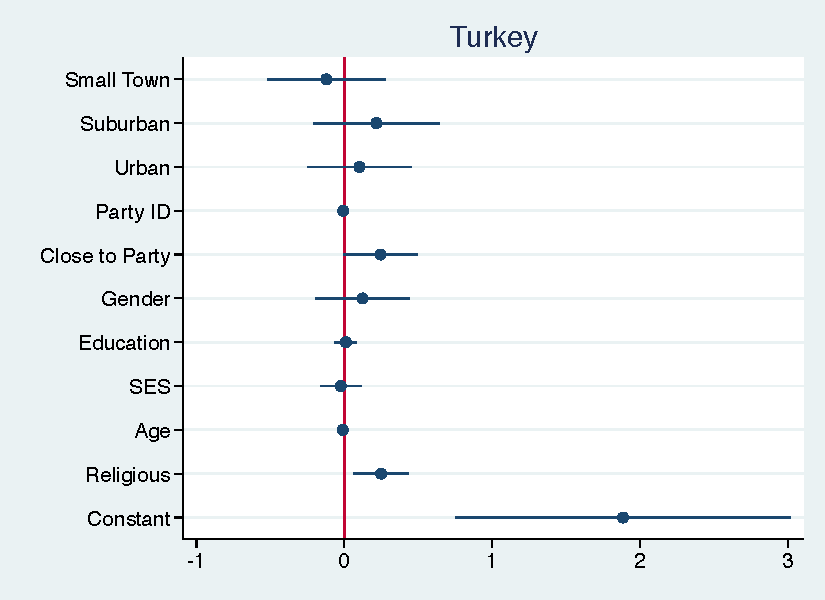
\includegraphics[width=\textwidth]{LibCoef/Turkey}
	\end{subfigure}
	\caption[ \tb{Issue Stances - Middle East} ]
	{\tb {Coefficient Plots for Issue Stances in Middle East} }
	\label{MidEastLibCoef}
\end{figure}

\begin{singlespace}
	\begin{table}[H]
		\centering
		%\def\arraystretch{1.5}
		\caption{\tb{Issue Stances - Africa}}
		\begin{tabulary}{\linewidth}{l c}

			\hline
			\tb{Place of Residence}& \tb{South Africa} \\
			\hline
			Urban&-.1861 \\
			&(.1871)\\
			Constant&1.989*** \\
			& (.6058) \\
			N& 220\\
			$R^2$&0.0544 \\
			\hline
		\end{tabulary}
		\\
		\e{Notes:} *p$<$.1, **p$<$.05. ***p$<$.01 \\
		\e{Reference:} A rural place of residence serves as the baseline for comparison
		\label{AfricaLib}
	\end{table}
\end{singlespace}

\begin{figure}[H]    \centering
	{	 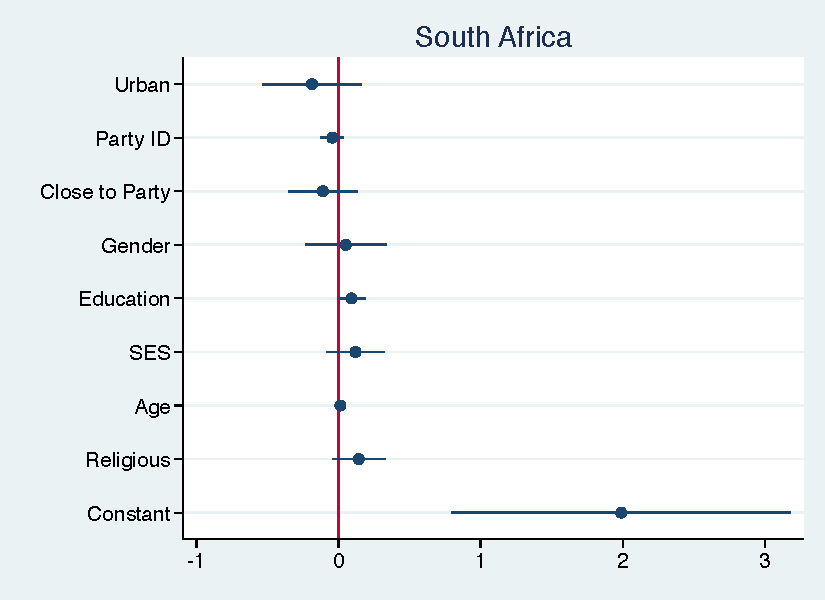
\includegraphics[width=.5\textwidth]{LibCoef/SAfrica}}
	\caption[ \tb{Issue Stances - Africa} ]
	{\tb {Coefficient Plots for Issue Stances in Africa} }
	\label{AfricaLibCoef}
\end{figure}

\begin{singlespace}
	\begin{table}[H]
		\centering 
		%\def\arraystretch{1.5}
		\caption{\tb{Issue Stances - Asia}}
		\begin{tabulary}{\linewidth}{l c c c}

			\hline
			\tb{Place of Residence} & \tb{Japan} & \tb{South Korea}&\tb{Thailand}\\
			\hline
			Small Town&.2140*&.2990* &-.0567 \\
			&(.1246)&(.1787)  & (.2647) \\
			Suburban&.2256* &.2952 &-.3755 \\
			&(.1307)&(.2937)  & (.4216) \\
			Urban&.1879&.2611  & .8547**\\
			&(.1209)& (.1602) & (.4216) \\
			Constant&3.1767***&2.0334***  & 3.6734*** \\
			&(.3418)& (.5822)  & (.6880) \\
			N&558&328  & 116  \\
			$R^2$&0.0337& 0.0494 & 0.1305 \\
			\hline
\end{tabulary}
\\
\e{Notes:} *p$<$.1, **p$<$.05. ***p$<$.01 \\
\e{Reference:} A rural place of residence serves as the baseline for comparison
\label{AsiaLib}
\end{table}
\end{singlespace}

%Fix Thailand Figure and Add to graphic later
\begin{figure}[H]
	\centering
	\begin{subfigure}[b]{0.475\textwidth}
		\centering
		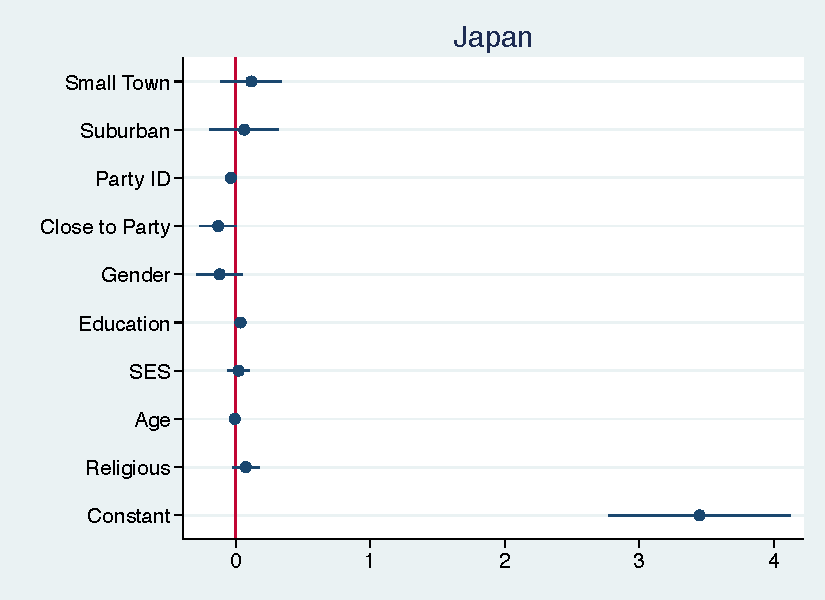
\includegraphics[width=\textwidth]{LibCoef/Japan}
	\end{subfigure}
	\hfill
	\begin{subfigure}[b]{0.475\textwidth}  
		\centering 
		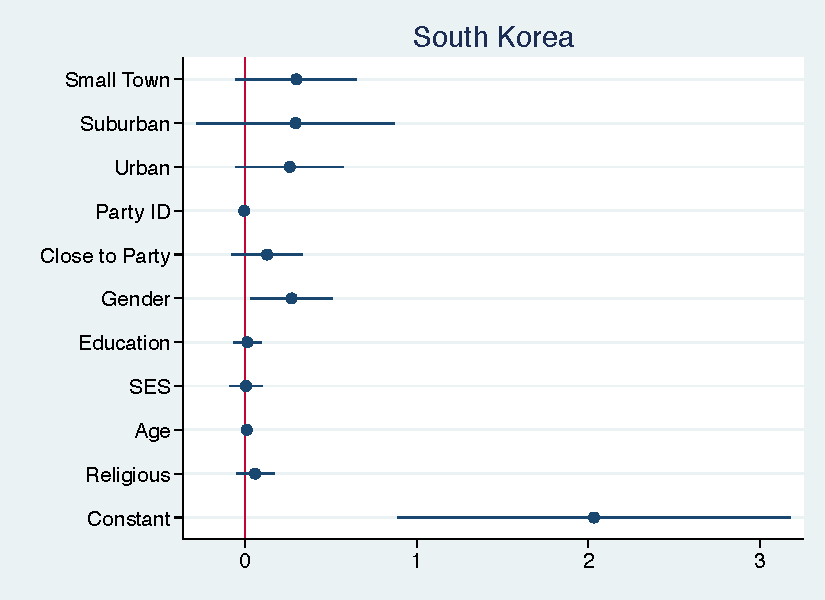
\includegraphics[width=\textwidth]{LibCoef/SKorea}
	\end{subfigure}
	\caption[ \tb{Issue Stances - Asia} ]
	{\tb {Coefficient Plots for Issue Stances in Asia} }
	\label{AsiaLibCoef}
\end{figure}

\begin{singlespace}
	\begin{table}[H]
		\centering
		%\def\arraystretch{1.5}
		\caption{\tb{Issue Stances - Pacific Islands}}
		\begin{tabulary}{\linewidth}{l c c }

			\hline
			\tb{Place of Residence}&\tb{New Zealand (2011)}&\tb{Philippines}\\
			\hline
			Small Town&-.2018*&-.5318* \\
			&(.1169)&(.3038) \\
			Suburban&- &-.3377 \\
			&-&(.5366) \\
			Urban&-.0508&-.5314*** \\
			&(.1141)& (.1808)\\
			Constant& 4.4689&4.4887*** \\
			&(.3239)& (.7104) \\
			N&565&112 \\
			$R^2$&0.0332& 0.2003 \\
			\hline
\end{tabulary}
\\
\e{Notes:} *p$<$.1, **p$<$.05. ***p$<$.01 \\
\e{Reference:} A rural place of residence serves as the baseline for comparison
\label{PacificLib}
\end{table}
\end{singlespace}

\begin{figure}[H]
	\centering
	\begin{subfigure}[b]{0.475\textwidth}
		\centering
		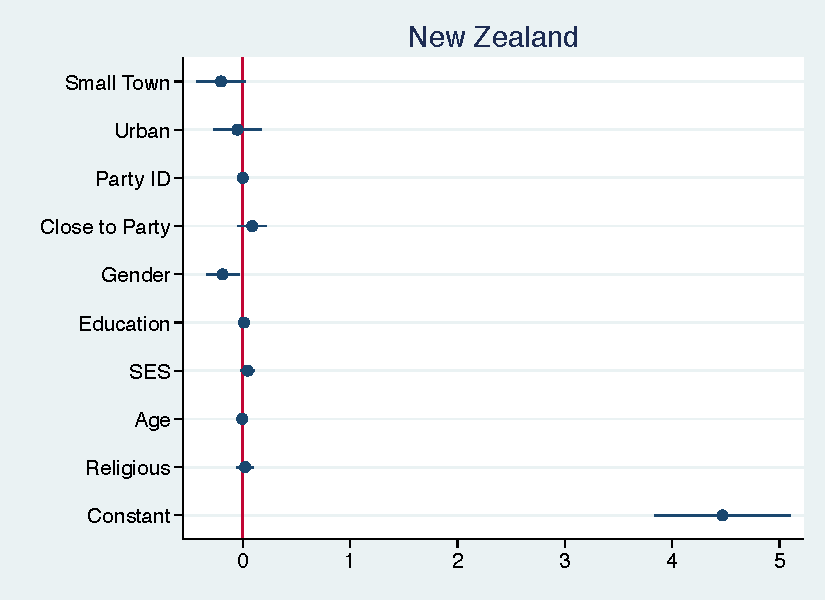
\includegraphics[width=\textwidth]{LibCoef/NZealand}
	\end{subfigure}
	\hfill
	\begin{subfigure}[b]{0.475\textwidth}  
		\centering 
		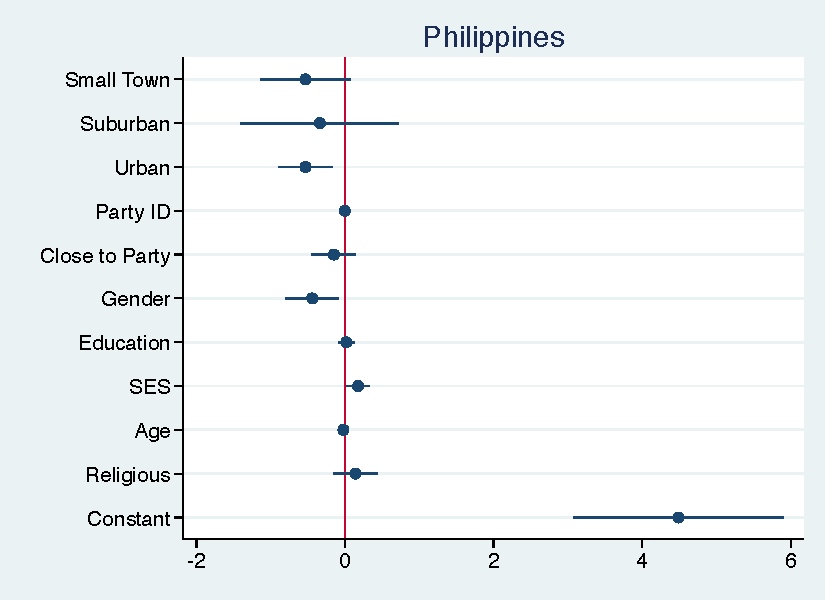
\includegraphics[width=\textwidth]{LibCoef/Philippines}
	\end{subfigure}
	\caption[ \tb{Issue Stances - Pacific Islands} ]
	{\tb {Coefficient Plots for Issue Stances in Pacific Island} }
	\label{PacificLibCoef}
\end{figure}

As we can see from these analyses relating to issue stances, place of residence matters but, like the results of the \e{Self-Identified Ideology} hypothesis, these vary widely across differences in level of democracy, regime age and electoral formula.

\subsection{Considerations of Regime Age, Level of Democracy, and Electoral Formula}

In the analysis of results for self-placement ideology, we considered if a country's macro variables has any influence on the relationship between place of residence and political ideology.

To test the core of Hypothesis 3, we will turn next to how these macro variables influence the context where each respondent casts their ballot. I will analyze the big picture before diving into the specifics regarding each factor. Therefore, we will look at the \e{Polity Difference} hypothesis before diving into \e{Level of Democracy}, \e{Regime Age}, and \e{Electoral Formula} hypotheses.

Table \ref{table15} shows the influence of each of the macro variables, when taken together, on the relationship between place of residence and individual placement on political ideology and on the objective measures seen in the liberalism scale.

%Self Placement and Liberalism Column Changed
\begin{table}[h!]
	\centering
	%\def\arraystretch{1.5}
	\caption{\tb{All Macro Variables - General Trends}}
	\begin{tabulary}{\linewidth}{l c c}

	\hline
	\tb{Variable}&\tb{Self-Placement}&\tb{Liberalism} \\
	\hline
	\e{Place of Residence} & & \\
	Small Town &.1301*&-.0275 \\
	&(..0736)&(.0269) \\
	Suburban& .0884& -.0741** \\
	&(..0976)& (.0347) \\
	Urban&.1484** & .0995*** \\
	&(..0751) & (.0266) \\
	\e{Democracy}& .1178***& .0030***\\
	&(..0357) & (.0120)\\
	\e{Regime Age} & -.0037** & .0035***\\
	&(..0016) & (.0005)\\
	\e{Electoral Formula}&-.0518& .0888***\\
	&(..0484) & (.0167) \\
	\e{Freedom House}& -.8108*** &-.0593*** \\
	&(.1065) & (.0340)  \\
	\e{Corruption Perception}&.0226***&.0148*** \\
	&(.0044)& (.0014)  \\
	\hline
	Constant& 7.928*** & 2.1065*** \\
	&(.4323) & (.1439)\\
	N&10,122 & 9,292 \\
	$R^2$&0.0509& 0.1113 \\
	\hline
	\end{tabulary}
	\\
\e{Notes:} *p$<$.1, **p$<$.05. ***p$<$.01 \\
\e{Reference:} A rural place of residence serves as the baseline for comparison
\label{table15}
\end{table}

\begin{figure}[H]
	\centering
	\begin{subfigure}[b]{0.475\textwidth}   
		\centering 
		\includegraphics[width=\textwidth]{IdeoMacroCoef}
		\caption{Self-Placement Ideology}
	\end{subfigure}
	\hfill
	\begin{subfigure}[b]{0.475\textwidth}
		\centering 
		\includegraphics[width=\textwidth]{LibMacroCoef}
		\caption{Issue Stances}
	\end{subfigure}
	\caption{\tb{Coefficient Plots - All Macro Variables Worldwide}}
	\label{GlobalMacroCoef}
\end{figure}

The data in Table \ref{table15} suggests that there is a difference between urban and rural residents when it comes to self-placement ideology and government spending. Despite the lower scores and levels of significance for the individual place of residence, we see that the macro variables are significant influences of the relationship between place and political ideology on their own. 

In the next sections, I run interactions with each of the macro variables listed under Hypothesis 3 along with the  Freedom House Ratings and Corruption Perception Index as independent and control variables to see how these factors influence the relationship of place and ideology. Appendix \ref{Online} contains the technical processes that were behind these calculations. 

\subsubsection{By Level of Democracy}

A model that considers the interaction between a person's place of residence and their country's level of democracy suggests that the level of democracy, alone, only differs slightly between places such that there is almost no effect between your country's level of democracy and where you live that will make a noticeable difference on your personal political ideology nor your feelings towards government spending.

The only noteworthy deviation is for countries scoring an 8 on the Polity IV democracy index. The people here are more likely to place themselves lower on the ideology spectrum, thus seeing themselves to be more left leaning as a whole. However, there do not see to be any place differences embedded into these general trends. 

\subsubsection{By Regime Age}

When it comes to regime age, countries younger than 50 years and older than 100 are more likely to have place differences in terms of both political ideology and government spending. As a regime gets older than 100 years, urban residents are more likely to lean more to the left when compared to their rural counterparts under the self-placement ideology scale. They are also more likely to favor government spending towards social welfare policies in these older regimes. 

In general, urban residents in countries with an established democracy of under 50 years tend to be more conservative, or right leaning, than their rural counterparts. This effect is also observed when we consider their preferences on government spending. The trends move towards zero, or no effect, as the regime nears 50 years and stays there until around 100 years. During this time, political attitudes are not affected by place, and may instead be impacted by another variable not considered in this study.

\subsubsection{By Electoral Formula}

%For this section, we consider Electoral formula. Since there are only 3 categories that any country can select, it makes direct comparison more straightforward. Unlike the previous two discussions, this variable is not continuous, thereby making interactions not as suitable.

%\begin{table}[h!]
%	\centering
%	\caption{\tb{Ideology In Each Electoral Formula}}
%	\begin{tabulary}{\linewidth}{l c c c}
%		\hline
%		\tb{Place of Residence}&\tb{Majoritarian}&\tb{Proportional} &\tb{Mixed} \\
%		\hline
%		Small Town&-.2413 &.3437*** &.0425 \\
%		&(.1583)&(.0982) &(.1377) \\
%		Suburban&-.0981 &.2715**&.4923**  \\ 
%		&(.2307) &(.1174) &(.2124) \\
%		Urban&-.3787* &.1999** &.5009*** \\
%		&(.1995) &(.0981) &(.1298) \\
%		Constant& 1.776*** &5.3337***&5.9321*** \\
%		&(.5730) &(.2616) &(.3651) \\
%		N&1,440&6,057 &3,043\\
%		$R^2$&0.1375&0.0549&0.0221 \\
%		\hline 
%	\end{tabulary} 
%\\ 
%\e{Notes:} *p$<$.1, **p$<$.05. ***p$<$.01 \\
%\e{Reference:} A rural place of residence serves as the baseline for comparison
%\label{table16}
%\end{table}

%Table \ref{table16} shows the relationship of place of residence in countries grouped by their electoral formula. By the differences in the results, we can see that the electoral formula matters in the relationship between place of residence and political attitudes.

Differences in the method of election can lead to differences in campaign strategies and voting styles. Therefore, the political ideologies of individuals can be based in the electoral system and political culture established and developed during a country's transition to democracy. 

Majoritarian elections are defined by first-past-the-post result tabulations where the candidate with the most votes is tapped as the winner of the race. With this campaign method, there is space of candidates to appeal to certain constituencies strategically to gain the most votes for themselves. In theory, a large representative body should serve different interests, but reality is hard to match expectations. Therefore, candidates and voters alike must push for their own interests to dominate, making a polarized electorate more likely on the lines of differing interest \cite{abramowitz-2010}. The results confirms this expectation. Individuals living in small towns, suburban and urban areas are more likely to lean left than their rural counterparts. However, only urban residents have statistical significance compared to their rural counterparts, but it is over a third of a point to the left, making that a moderate influence. Despite the aggregated statistical significance, it is also important to note that this pattern is not present for all majoritarian systems when broken down. The only country where this same pattern is seen is in France. Other majoritarian countries may see a move in this general direction, but not to the extent of statistical significance.

Proportional representation occurs when parties are able to allocate votes in ratio to the number of votes that they receive. Therefore, it becomes more likely that different interests are represented in practice and that minority parties will have a chance in policy-making. Yet the results suggest that there is a mild rural-urban divide among the respondents, and this effect is present in all areas of residence studied in this analysis. From the results, we see that there is a trend towards conservatism, even if it is more pronounced in small towns compared to rural areas than in urban centers compared to rural areas. Yet, while the aggregate tells this picture, there are also proportional systems that confirm the \e{Self-Identified Ideology} hypothesis, namely Greece in 2012 and South Africa. There are proportional systems that may move in the direction of the aggregate but the observations may occur due to chance.

Finally, a mixed representation system has combinations of the aforementioned systems. When aggregated, there are differences between place of residence and political attitudes. Much like the results in a proportional system, the responses for urban residents are over a half a point to the right, which is a relatively significant amount for countries in this system. This trend goes against the observations of Mexico in their 2015 election, even if it confirms the patterns of Romania in 2012. 

To conclude, we see that the electoral formula matters in shaping political competition and electoral appeals from the perspective of the party. However, there are not clear distinctions for formulas such that it is a tell-all third factor in explaining the relationship between place and political attitudes. When aggregated, we find differing results than when the countries are broken down, showing that an aggregation of an effect does not indicate how the specifications of polity uniqueness may play out.

\subsubsection{Freedom House Ratings and Corruption Perception Index}

As mentioned earlier in this paper, Freedom House Ratings and the Corruption Perception Index score for each country was included in this analysis model to control and understand how each country meets the criteria for a free and fair democracy as defined by \cite{diamond2004overview}. To understand the freedom, equality and responsiveness principles, I include these variables both as controls and as independent variables to see how they themselves would interact with place of residence to influence one's political ideology and attitudes towards government spending. 

The Freedom House Rating is made by the Freedom House and it measures the extent of political freedoms and civil liberties one has in their country. This ranges from 1, being the least free to 7, which is the most free. The range does not reflect the original rankings; rather these are recoded for the analysis and interpretation to match the direction of the other scales used in this paper.  In the regression model where I interacted this rating with place of residence to see how this would influence individual political ideology and attitudes towards government spending on social welfare issues. From the results, there does not seem to be an interaction between the variables. In other words, the freer a country, the less that this freedom influences the differences in opinions between place of residence and political ideology. While there are differences between place, the effect cannot be fully attributed to place of residence.

The Corruption Perception Index was added as a means to understand government responsiveness to the desires to the citizens. In a more corrupt nation, the leaders on top are less likely to respond to popular desires and cater to the needs and interests of their own leaders. This scale ranges from 0, being the most corrupt to 100, being the least corrupt. Across all levels of corruption, urban residents consistently differ from their rural counterparts in terms of views towards government spending, such that they are more likely to be more conservative about it. However, this is not seen in the scores related to the self-placement on the ideology scale. Where there are slight differences between place of residence everywhere, this effect is not noticeable enough to have a large impact.

Therefore, from these analyses, the placement of the Freedom House Rating and the Corruption Perception Index is helpful in controlling for regime differences in these factors and allowing for a more uniform definition of democracy, but these factors themselves do not carry that big of an effect on how place influences political ideologies and issue attitudes. 

Taken together, the analyses in this section suggest that when each of these macro variables are alone, they may produce effects not observed by chance, but they can also produce some interactive effects with the place of residence variable. The null results in this section suggests that not one polity defining variable can work to produce significance in its influence of the relationship between place and political ideology. This is an effect that can lead to future research to understand how the variables cooperate to create effects. While I was not able to gain an understanding of overall cooperative effects of the five macro variables, the regressions for each individual country suggests that there are still variations between the polities beyond these five that can determine whether there is a place difference for political ideology and issue attitudes. 

\section{General Discussion and Conclusion}

From the results of the data analyses, we can see that there are general relationships between place and political attitudes. However, when we dive deeper into the individuality of each country, we see that the idiosyncrasies that define each polity makes this a hard generalization to make. 

\subsection{Summary of Findings}

The goal of this paper is not to make generalizations about how people who live in suburbia around the world compare to those in the rural countryside when it comes to political attitudes, rather, it is to gain a general understanding of how the variables of place and political attitudes relate on a broad and specific level. From the data, I can draw the following conclusions. First, place matters. In the \e{Self-Identified Ideology} hypothesis, the results confirm the findings such that urban residents, on average, differ from their rural counterparts when it comes to political ideology. However, the results does not support the predicted general direction of the hypotheses. Unlike the results shown in past literature, many countries tend to lean right, with the exception of Greece.

Second, the \e{Issue Stances} hypothesis is supported by the data because a person's place of residence does influence how one conceptualizes the issues and rate their support. However, as seen in Table \ref{table14}, urban residents are, on average, more conservative on their willingness to spend public dollars than their rural counterparts. This comes in contrast with the results in the \e{Self-Identified Ideology} hypothesis. While urban residents may see themselves as more left leaning, they may have other motivations to limit their support for social and economic policy.

Finally, in Hypothesis 3, we examine the macro variables that are part of defining major democratic aspects of each country. We find that the \e{Polity Differences} hypothesis holds, but to a rather limited extent for both dependent variables. When these factors are included in a model along with Freedom House Rating and Corruption Perception Index, the results suggest that these variables are contributing factors to how the worldwide trends operate in the ability for people in different places of residence to express their political attitudes. However, individually, there are limited differences between levels in each factor and its role in the relationship between the variables. We have some reason to suggest that these factors are cooperating in each country to influence the trends of influence between place and political attitudes, yet this would have to be proven through future research.

While there are significant results to demonstrate that place of residence matters, there are many other variables that may play into the extent to which place matters in each polity.

\subsection{Limitations and Future Directions}

For this project, that are many possible future directions that the research can go. In this section, I discuss how present limitations can become possible access points to future research and expansions of this paper.

As discussed throughout the analysis, each polity's idiosyncrasies cannot be fully accounted for in this one study. While this study is useful in understanding global trends, more research in the country's macro-variables are necessary to understanding why there is a significant relationship between place and political ideology in some counties and not others, even if they share grounds on level of democracy, regime age, and electoral formula.

The liberalism issue stance scale was created as a means of universalism, which was helpful in gaining some insight on how individuals conceptualize issue stances. However, it would be helpful to take the voting behavior of each participant into account and see how their self-rated political ideology compares to the candidate that they voted for in their legislative election. These specifications that are necessary to understand the differences between polities for the relationship of place and political attitudes provides insight as to why case studies have been the more popular method in analyzing these trends. 

While there is a relatively healthy mix of countries from different regime ages and electoral formulas, there is not an even distribution of countries based on their level of democracy. For future research, it would be helpful to include more transitioning regimes and autocratic regimes so long as public data is available. It is hard to gather data in their regimes due to government limitations, but trends in these sections would be interesting to observe.

Nonetheless, future research can be dedicated to looking at specifications that set each polity aside including historical, economical, political and other social factors. Residents of a certain place, as \cite{holloway_burning_2007} noted, are clearly not voting blocs. Unique factors of each country can help to explain the influence, or lack thereof, of place and political ideology better than how generalizations can tease out.       

\clearpage


%\let\svaddcontentsline\addcontentsline
%\renewcommand\addcontentsline[3]{%
%	\ifthenelse{\equal{#1}{lof}}{}%
%	{\ifthenelse{\equal{#1}{lot}}{}{\svaddcontentsline{#1}{#2}{#3}}}}


\appendixtitleon
\appendixtitletocon

\begin{appendices}
	
\section{The 2016 US Presidential Election}
\label{AppendixE}

Figure \ref{figure3} shows the distribution of voters for Donald Trump and Hillary Clinton by county in the United States in 2016 as reported by the  \cite{NYT-trump}.

\begin{figure}[H]    \centering
	{	 \includegraphics[width=\textwidth]{NYT}}
	\caption{\tb{Distribution of Trump and Clinton Voters in 2016}}\label{figure3}
\end{figure}	

\clearpage

\section{Regimes Broken Down by Macro Variables}
\label{AppendixC}

\begin{table} [h!]
	\centering
	\caption{\tb{Regimes by Level of Democracy, Regime Age, and Electoral Formula}}
	\begin{tabulary}{\linewidth}{l c c c}
		\hline
		\tb{Country} & \tb{Level of Democracy} & \tb{Age of Regime} & \tb{Electoral Formula} \\
		\hline
		Argentina&9&32&Proportional \\
		Australia& 10&112&Majoritarian \\
		Austria&9&24&Proportional\\
		Bulgaria&8&24&Proportional\\
		Canada (2015)&10&127&Proportional\\
		Czech Republic&9&20&Proportional \\
		Finland&10&71& Proportional \\
		France&9&43&Majoritarian \\
		Germany&10&23&Mixed \\
		Great Britain&10&135&Majoritarian \\
		Greece (2015)&10&40&Proportional \\
		Ireland&10&90&Proportional \\
		Israel&10&60&Proportional \\
		Japan&10&61&Mixed\\
		Kenya&9&11&Majoritarian \\
		Latvia (2014)&8&23&Proportional\\
		Mexico (2015)& 8&18&Mixed\\
		Montenegro&9&6&Proportional\\
		Norway&10&68&Proportional\\
		New Zealand (2014)& 10& 137& Mixed\\
		Peru&9&15&Proportional\\
		Philippines&8&26&Majoritarian\\
		Poland&10&20&Proportional\\
		Portugal&10&39&Proportional\\
		Romania (2014) &9&18& Mixed \\
		Serbia& 8&6&Proportional\\
		Slovakia&10&23&Proportional\\
		Slovenia&10&20&Proportional\\
		South Africa&9&20& Proportional \\
		South Korea&8&24&Mixed\\
		Sweden&10&97&Proportional\\ 
		Switzerland&10&163&Proportional\\
		Turkey&3&32&Proportional\\
		United States&10&203&Majoritarian \\
		\hline
	\end{tabulary}
\\
\e{Source:} Polity IV Project and CSES Macro Report
\label{table101}
\end{table}

\clearpage 

\begin{landscape}
\section{Descriptions of Variables }
\label{AppendixA}

~~~\\

\begin{table}[h!]
	\centering
	\def\arraystretch{1.3}
	\caption{\tb{Variables Used in Analyses}}
	\begin{tabulary}{\linewidth}{l c c c}
		\\
		\hline
		\tb{Variable Name}& \tb{Variable Number} & \tb{Description}&\tb{Outside Source} \\
		\hline
		Election ID Variable &D1004&Polity and Election Year&-\\
		Place of Residence&D2031&Rural or Urban Residence&-\\
		Left-Right Self&D3014&Self-rate ideology &-\\
		Age&D2001\_Y&2018-VAR-Value&- \\
		Gender&D2002&Gender of Respondent&- \\
		Education&D2003&Highest Education Attained&- \\
		Socioeconomic Status&D2012&SES&- \\
		Religiosity&D2025&Identifies with religion?&-  \\
		Party ID&D3018\_3&Party Closest to R&- \\
		Closeness&D3018\_4&Party attachment&- \\
		Level of Democracy&D5051\_1&Democracy-Autocracy at Election&Polity IV Project\\
		Age of Current Regime&D5052&Age of Regime in Years& Polity IV Project\\
		Electoral Formula&D5058&Method of Election&CSES Macro Report\\
		Freedom House Rating&D5050\_1&Political Freedom/Civil Liberties&Freedom House \\
		Corruption&D5086&Corruption Perception Index&Transparency International \\
		\hline
	\end{tabulary}\\
	\e{Source:} Comparative Study of Electoral Systems Module IV Codebook available at \url{http://www.cses.org/datacenter/module4/data/cses4_codebook_part2_variables.txt}
	\label{table99}
\end{table}

\begin{table}[h!]
	\centering
	\def\arraystretch{1.5}
	\caption{\tb{Issue Stances/Liberalism Scale Variables}}
	\begin{tabulary}{\linewidth}{l c c c}
		\\
		\hline
		\tb{Variable Name}& \tb{Variable Number} & \tb{Description}\\
		\hline
		Health&D3001\_1&More or Less Public Expenditure on Health\\
		Education&D3001\_2&More or Less Public Expenditure on Education\\
		Unemployment Benefits&D3001\_3&More or Less Public Expenditure on Unemployment\\
		Defense&D3001\_4&More or Less Public Expenditure on Defense\\
		Old-Age Pensions&D3001\_5&More or Less Public Expenditure on Pensions\\
		Business and Industry&D3001\_6&More or Less Public Expenditure on Businesses\\
		Police&D3001\_7&More or Less Public Expenditure on Law-Enforcement\\
		Welfare Benefits&D3001\_8&More or Less Public Expenditure on Welfare\\
		Income Inequality&D3004&Should Government do more for Income Inequality?\\
		\hline
	\end{tabulary}\\
	\e{Source:} Comparative Study of Electoral Systems Module IV Codebook available at \url{http://www.cses.org/datacenter/module4/data/cses4_codebook_part2_variables.txt}
	\label{table100}
\end{table}

\end{landscape}
\clearpage

\section{Creation of the Issue Stances/Liberalism Scale}
\label{AppendixB}

\subsection{Variable Selection}

The CSES provides several issue stance items that reflect how individuals feel toward political parties and policies. The variables described in Table \ref{table100} show the variables that were selected as part of the liberalism scale because it reflects rather universal issues that are at the core of what citizens in each country would have to decide on in terms of the way they see their government spending their tax dollars. Additionally, each of these variables are focused on identifying how individuals feel about certain social issues based on their level of comfort in allocating money to the particular cause. As a results, we can see ther interaction of economic and social policy attitudes at work and see how they interact with place to build a person's ideology.

\subsection{Variable Coding}

The CSES codes the public expenditure variables (D3001) as follows:

\begin{quote}
	
	1. Much more than now \\ 
	2. Somewhat more than now \\
	3. The same as now \\ 
	4. Somewhat less than now \\
	5. Much less than now \\
	7. Volunteered: Refused \\
	8. Volunteered: Don't Know \\
	9. Missing

\end{quote}

For each of the variables, the response corresponding to the intention that an individual would be very willing to see the government spend more money on a particular issue (such as better health care), would be coded as 1 for most liberal. This scale places the most conservative at 0, meaning that the individual does not want government to step in to influence the particular matter. Some of the variables are reverse coded to reflect conservatives' typical greater favoritism towards increased defense spending or other factors that would make one's country look stronger in reference to others. Each of the answers in the middle are scaled accordingly between 0 and 1. Any refusals to answer the question, don't knows and missing answers are all treated as missing data and excluded from the research analysis.

Additionally, the CSES codes the variable on income inequality (D3004) as follows: 

\begin{quote}

	1. Strongly agree \\
	2. Somewhat agree \\
	3. Neither agree nor disagree \\
	4. Somewhat disagree \\
	5. Strongly disagree \\ 
	7. Volunteered: Refused \\
	8. Volunteered: Don't Know \\
	9. Missing
\end{quote}	

This income inequality follows the same recoding logic as the public expenditure items that preceded it. In these cases, an individual who would be most willing to see the government do something to curtail income inequality would be coded as 1 for most liberal, and someone who would not want the government to step in to fix the issue at all would be coded as 0, for most conservative. Like the previous variables, the answers in the middle are scaled accordingly and all refusals in answer, don't knows, and missing responses are treated as missing data.

Additionally, it is important to note that not all respondents of all countries were asked each of the questions. Therefore, if applicable, the countries that are missing one of the nine variables are also omitted from the analysis

\subsection{Liberalism - Variable Generation}

The \txt{liberalism} variable was generate by an aggregation of the 9 questions. Each of the variables were recoded and summed. The final score yielded a 0-9 scale where a person who scored a 9 is evaluated as the most conservative in terms of their view on economic and social policy, whereas someone with a score of 0 would be the most opposite.

\clearpage 


\section{Dependent Variables -- General Trends}
\label{AppendixD}

The tables depicting general trends are reproduced below for an easier side-by-side comparison.

\begin{singlespace}
	\begin{table}[H]
		\centering
		%\def\arraystretch{1.5}
		\caption{\tb{Worldwide Political Issue Attitudes - Two Measures}}
		\begin{tabulary}{\linewidth}{l c c}
			\\
			\hline
			\tb{Place of Residence}&\tb{Self-Placement}&\tb{Liberalism} \\
			\hline
			Small Town&.1647**&.0432  \\    
			& (..0722) &(.0278)  \\
			Suburban & .2714*** &.0082\\ 
			& (.0934) &(.0352) \\
			Urban   & .2679*** &.0995***  \\
			& (.0721)  &(.0272)  \\
			Constant   & 5.1086*** &2.7915*** \\
			&(.1993)&(.0762)  \\
			N  & 10,548 &9.662  \\
			$R^2$	& 0.0454&0.0195 \\
			\hline                                       
		\end{tabulary}
		\\
		\e{Notes:} *p$<$.1, **p$<$.05. ***p$<$.01 \\
		\e{Reference:} A rural place of residence serves as the baseline for comparison
		\label{table102}
	\end{table}
\end{singlespace}
\clearpage

\section{For Further Information and Reproductions}
\label{Online}

This paper contains some additional graphs and reproduction information that would not fit on this paper for length and size concerns. Therefore, these materials are attached in the form of a Git Repository for reference and reproduction.

The data for this project can be downloaded from the CSES Module IV page: \url{http://www.cses.org/datacenter/module4/module4.htm}

All of the Stata DO files and process-flow for this paper can be accessed by cloning this Git Repository link to a local device: \url{https://github.com/lin-jennifer/CompRuralPolitics.git}

There are five different Online Appendices Files that are attached to this document, and it is available on the Git Repository as a .tex and .pdf format. Additionally, they are available by clicking each name below.

\begin{quote}
\href{https://drive.google.com/file/d/175fvnZSjtcPDN4PoS1wW_Iw-PWTRWVJk/view?usp=sharing}{Online Appendix A -- Box Plots as Summary Statistics for Each Country} \\
\href{https://drive.google.com/file/d/1rFyIFRxbDp8NFk02RaVUj-C6hNtOKx2u/view?usp=sharing}{Online Appendix B -- Residual Plots for Regressions} \\
\href{https://drive.google.com/file/d/15xRxKmMw7UeUlXWFSc1yJr_eGSFOcDjU/view?usp=sharing}{Online Appendix C -- Margins Plots for Macro Variable Interactions} \\
\href{https://drive.google.com/file/d/1OVcB038erJnrL_R9ExDKx5ryF-qSXKyp/view?usp=sharing}{Online Appendix Y -- ARCHIVE Draft 1 of Results}  \\
\href{https://drive.google.com/file/d/1byaS6KsEFQO-ZLMpMFtgMAwa7bZ1pzXR/view?usp=sharing}{Online Appendix Z -- ARCHIVE Elections held by each country in CSES} \\
\end{quote}

\clearpage

\end{appendices}


\clearpage
\bibliography{RuralPolitics}
\bibliographystyle{chicago}


\end{document}
